\documentclass[economies,article,submit,moreauthors]{Definitions/mdpi}

\usepackage{threeparttable}
\usepackage{makecell}
\usepackage{xurl}

\firstpage{1}
\makeatletter
\setcounter{page}{\@firstpage}
\makeatother
\pubvolume{1}
\issuenum{1}
\articlenumber{0}
\pubyear{2026}
\copyrightyear{2026}
\datereceived{}
\daterevised{}
\dateaccepted{}
\datepublished{}

\Title{An Empirical Analysis of the Impact of the Digital Economy on Carbon Emissions: Evidence from China's Provincial Panel Data}

\newcommand{\orcidauthorA}{0009-0009-5504-3079}

\Author{Mingyu Fan $^{1}$\orcidA{} and Yile Wang $^{1,}$*}

\AuthorNames{Mingyu Fan and Yile Wang}

\address{%
$^{1}$ \quad School of Economics, Beijing Technology and Business University, Beijing 102488, China; 2401050107@st.btbu.edu.cn (M.F.); 2401050128@st.btbu.edu.cn (Y.W.)}

\corres{Correspondence: 2401050128@st.btbu.edu.cn}

\abstract{China's pursuit of peak carbon and carbon neutrality has coincided with the rapid expansion of the digital economy, yet whether digitalization alleviates or intensifies carbon pressure remains contested. This study examines the relationship using a balanced panel of 30 Chinese provinces from 2011 to 2022 ($N=360$). We construct a digital economy index (DEI) from 13 indicators and a carbon emission pressure index (CEI) from four indicators, combining entropy weighting with CRITIC--Spearman weighting; principal component analysis (PCA) provides alternative measures. Because both indices are right-skewed, we estimate log--log two-way fixed-effects models, supplemented by spatial Durbin models and system GMM. The baseline elasticity is $-0.278$ ($p<0.01$): a 1\% increase in DEI is associated with a 0.278\% decrease in CEI, and a 10\% increase with about a 2.8\% decrease. The negative association survives PCA replacement, lagged DEI, exclusion of municipalities, and winsorization, although it is concentrated in the composite pressure index rather than its carbon-intensity component. Energy efficiency is the stronger mechanism, with support at both links (elasticity 0.336); industrial structure upgrading is positively associated with DEI at the first link (elasticity 0.247). Spatial spillovers are negative and significant under economic-distance weights (indirect effect $-0.364$), but not under administrative contiguity. Regional heterogeneity is visible in the western subsample (elasticity $-0.688$), while the interaction model does not reject homogeneity. Carbon pressure is highly persistent (0.919). The estimates show that measurement and neighbor definitions shape conclusions, and that digitalization should be paired with energy-efficiency and green-computing policies.}

\keyword{digital economy; carbon emission pressure; log--log model; measurement robustness; spatial Durbin model; China}

\JEL{Q56; O33; C33; R12}

\makeatletter
% Local fix: the class places the first-page metadata column inside the text
% block with this TeX installation; shift it back into the left margin.
\let\mdpi@contentleftcolumn\contentleftcolumn
\renewcommand{\contentleftcolumn}{\hspace*{-5.87cm}\mdpi@contentleftcolumn}
\makeatother

\begin{document}

\section{Introduction}

China's commitment to peak carbon emissions before 2030 and reach carbon neutrality before 2060 has turned low-carbon transition into a national development constraint \citep{state2021}. In parallel, the digital economy has become a core engine of growth; digital infrastructure, digital industry, and digital inclusive finance now shape how provinces produce, trade, and consume \citep{tapscott,g20}. The two agendas are not automatically compatible. Data centers, networks, and digital devices are large electricity users, and efficiency gains can be offset by scale expansion. Whether digitalization lowers carbon pressure, and under which measurement and spatial conditions, remains an empirical question.

Recent provincial and city-level studies mostly report a negative association between the digital economy and carbon emissions or carbon intensity. \citet{gao2024} find that digital development reduces energy and carbon emissions, with common prosperity as a mediating channel. \citet{zhang2025} find that the digital economy lowers carbon emission intensity through direct and indirect channels, with spillovers concentrated within about 500 km. \citet{huangwu2024} and \citet{zhang2024sust} report similar reductions, working through green technology innovation and industrial upgrading. \citet{song2024}, \citet{yuan2024}, \citet{wang2025}, and \citet{niu2024} extend the evidence to spatial dependence and regional heterogeneity. A recent review, however, emphasizes that measurement, nonlinearity, and the energy intensity of digital infrastructure can generate heterogeneous conclusions \citep{liuwang2025}. The net association is therefore an empirical object, not a theoretical constant.

Three gaps motivate this study. First, composite indices are right-skewed and most studies fix one weighting scheme and one functional form, so it is unclear how much of the estimated association is a measurement artifact. Second, mechanism tests often rely on stepwise mediation, which treats the mediator as an exogenous control. Third, spatial studies often report one weight matrix, which makes it difficult to separate geographic clustering from economic diffusion.

We address these gaps with a balanced panel of 30 Chinese provinces from 2011 to 2022. We build a digital economy index (DEI) from 13 indicators and a carbon emission pressure index (CEI) from four indicators, combine entropy and CRITIC--Spearman weights \citep{shannon1948,diakoulaki1995}, and cross-validate the results with PCA measures. Because both indices are right-skewed, we estimate log--log two-way fixed-effects models, then spatial Durbin models under two neighbor definitions and system GMM. The baseline elasticity is $-0.278$ ($p<0.01$): a 10\% increase in DEI is associated with about a 2.8\% decrease in CEI. The association survives PCA replacement, lagged DEI, exclusion of municipalities, and winsorization. Energy efficiency is the stronger mechanism; spatial spillovers appear only when neighbors are defined by economic distance. Regional heterogeneity is visible in the western subsample but not in the interaction model.

The paper contributes in three ways. It shows that the sign of the digital economy--carbon relationship is robust to combined weighting versus PCA, but the magnitude is attenuated by measurement error. It shows that energy efficiency carries the mechanism through both links, while industrial structure matters at the first link. It shows that spillover conclusions depend on the neighbor definition: geographic contiguity captures the clustering of carbon pressure, whereas economic distance captures the diffusion of digital technology along industrial linkages. Section 2 reviews the literature and states the hypotheses. Section 3 describes the data and methods. Section 4 reports the results. Section 5 discusses implications and scope, and Section 6 concludes.

\section{Literature Review and Hypotheses}

\subsection{Digital Economy and Carbon Emissions: Empirical Evidence and Open Questions}

The digital economy is an economic system in which digital knowledge and information are key production factors, modern information networks are the main activity space, and information and communication technologies drive efficiency and structural change \citep{tapscott,g20}. It is usually measured along three dimensions: digital infrastructure, digital industry, and digital inclusive finance \citep{guo2020report}. This multidimensionality matters: a province can score high on infrastructure but low on industrial application, and different weighting schemes can produce different rankings and elasticities.

Recent empirical work on China generally finds that digital development reduces carbon emissions or carbon intensity. \citet{gao2024} report that digital development lowers energy and carbon emissions, with common prosperity as a mediating channel. \citet{zhang2025} find that the digital economy reduces carbon emission intensity through direct and indirect channels, with spillovers concentrated within about 500 km. \citet{huangwu2024} and \citet{zhang2024sust} identify green technology innovation and industrial upgrading as channels, and \citet{song2024} report a negative association in a provincial panel.

The literature also points to two boundary conditions. First, digital infrastructure is energy-intensive, and the net effect depends on how digital activity is powered and organized \citep{liuwang2025}. Second, the relationship may be nonlinear: digital development can have threshold effects, and the marginal effect may decline as the digital level rises \citep{zhang2024sust,zhang2025}. These studies establish a negative association, but they do not establish how much of it depends on measurement. Most rely on a single weighting scheme and a single functional form; when the composite index is right-skewed, a level-value semi-elasticity depends on the arbitrary units of the index and can be dominated by a few high-digitalization provinces. A log--log specification converts the relationship into a unit-free elasticity that uses proportional variation, and the PCA measures in Section 3.5 provide an alternative to the combined weights. We therefore test the following baseline hypothesis:

\textbf{H1.} Digital economy development is negatively associated with carbon emission pressure.

\subsection{Transmission Channels: Structural Change and Technical Efficiency}

The mechanisms linking digitalization to carbon pressure map onto the two classic channels in environmental economics: the composition effect and the technique effect \citep{grossman1991}. Digitalization changes what is produced by enabling service-oriented production and lowering the share of energy-intensive manufacturing; it changes how output is produced by improving monitoring, scheduling, and grid dispatch. We operationalize the two channels as industrial structure upgrading and energy efficiency.

Most mechanism tests treat the mediator as an exogenous control, which removes the part of the association that runs through the channel and makes the two channels hard to compare within one sample \citep{imai2010,bullock2010}. We therefore test each channel separately with a two-step design and compare their first links.

\subsubsection{Industrial Structure Upgrading as a Composition Channel}

Digitalization lowers search and matching costs, expands market access for services, and allows firms to separate production from service activities \citep{goldfarb2019}. These forces shift output from secondary to tertiary sectors, which are typically less energy-intensive per unit of value added. In China, digital development is positively associated with industrial structure upgrading \citep{huangwu2024,zhang2025}. Whether this shift lowers carbon pressure, however, depends on the energy intensity of the expanding service subsectors and on whether industrial relocation displaces emissions rather than reducing them. The channel therefore has to be traced at both links, from digitalization to the service share and from the service share to carbon pressure. This ambiguity motivates the first channel hypothesis:

\textbf{H2a.} Digital economy development is positively associated with industrial structure upgrading, which is in turn negatively associated with carbon emission pressure.

\subsubsection{Energy Efficiency as a Technique Channel}

Beyond changing what is produced, digitalization changes how output is produced. Digital energy-management systems, industrial internet platforms, and smart grids reduce energy input per unit of output by improving scheduling, reducing idle capacity, and detecting losses. The technique effect operates at the plant level, through real-time optimization, and at the system level, through demand-side management and renewable integration. Recent evidence shows that the digital economy improves urban energy efficiency \citep{ma2024} and raises energy productivity across Chinese provinces \citep{wang2025energy}. Part of the gain can be offset by rebound effects, because cheaper energy services encourage additional use \citep{gillingham2016}. Because efficiency improvements can be implemented within existing production units, while structural change requires reallocation across sectors, the technique effect may be the more proximate channel in the short run. This asymmetry motivates a separate test of the technique channel:

\textbf{H2b.} Digital economy development is positively associated with energy efficiency, which is in turn negatively associated with carbon emission pressure.

\subsubsection{Why Test Both Channels?}

Testing both channels within one framework serves two purposes. First, it allows a comparison of their relative magnitudes, which is policy-relevant: if the technique effect dominates, policy should prioritize digital energy management; if the composition effect dominates, policy should focus on service-sector upgrading. Second, the channels are not independent, because structural change can itself raise aggregate energy efficiency by shifting weight toward less energy-intensive sectors. Estimating each channel separately avoids conflating their contributions, while reading them side by side keeps their interdependence visible. For each channel we test the first link and rely on the cited evidence for the second.

\subsection{Spatial Spillovers: Geographic Clustering vs.\ Economic Diffusion}

Digital technology crosses provincial borders through trade in digital services, investment by digital firms, labor mobility, and supply-chain coordination. If these channels dominate, the relevant ``neighbor'' is an economic peer rather than a geographic neighbor. \citet{yuan2024} find a negative spatial spillover of the digital economy on neighboring provinces' carbon emissions; \citet{wang2025} and \citet{niu2024} report significant spatial effects, with the latter emphasizing equity implications. \citet{zhang2025} find that spillovers are strongest within a limited distance range.

However, the existing spatial evidence is almost entirely based on a single weight matrix, typically geographic contiguity or geographic distance. With one matrix, a detected spillover cannot be separated into geographic clustering of carbon pressure and economic diffusion of digital technology. To distinguish the two processes, we estimate the spatial Durbin model under two neighbor definitions---a composite weight that combines administrative contiguity with economic similarity, and a pure economic-distance weight---and compare their indirect effects:

\textbf{H3.} Digital economy development has negative spatial spillovers on carbon emission pressure in neighboring provinces, and the estimated spillover depends on whether neighbors are defined by administrative contiguity or economic distance.

Figure \ref{fig:framework} summarizes the framework and the design. The digital economy can affect carbon pressure directly (H1), through industrial structure upgrading (H2a) or energy efficiency (H2b), and through spillovers to other provinces (H3). The figure traces how each link is estimated, which results survive the stress tests, and how the robust core translates into policy.

\begin{figure}[!htbp]
\centering
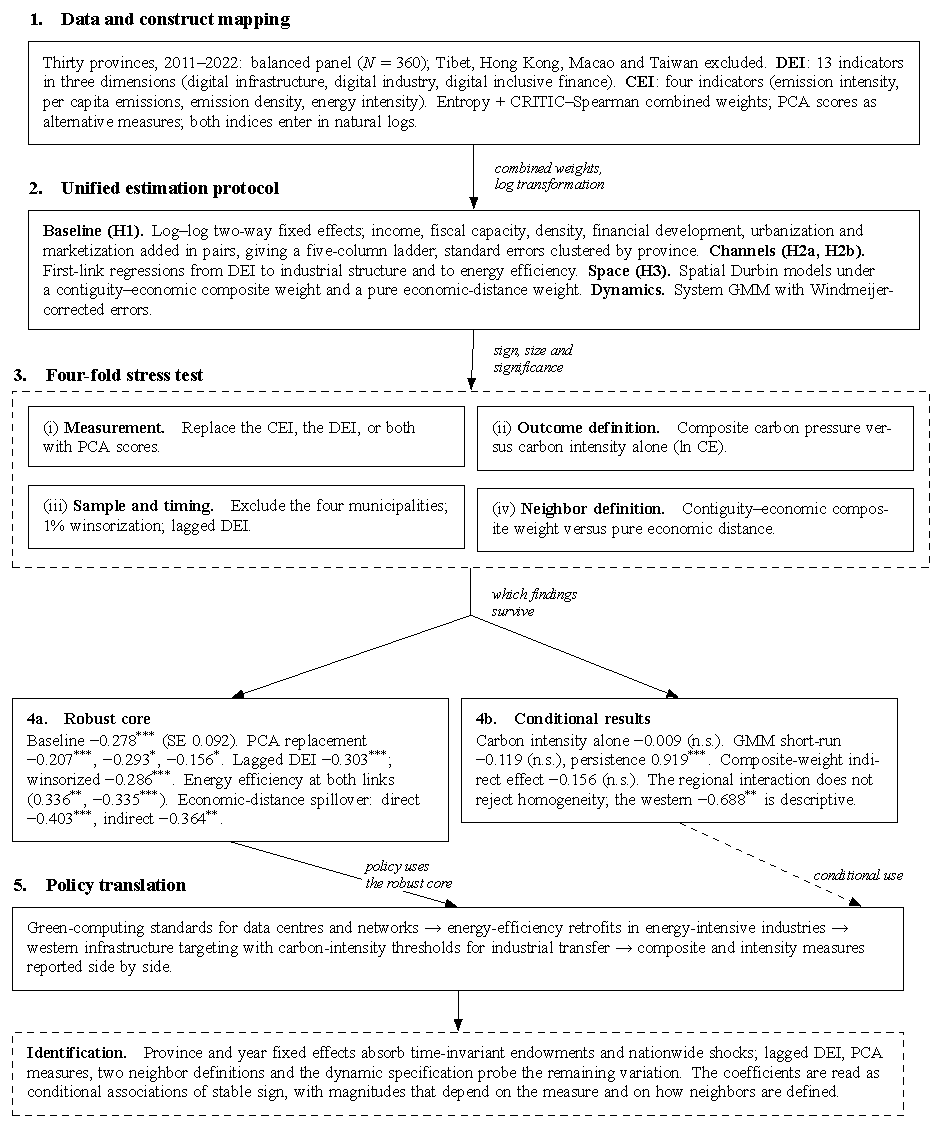
\includegraphics[width=\textwidth]{figures/fig01_framework.pdf}
\caption{The design of the paper as a single chain: 30 provinces and two composite indices enter a unified estimation protocol; the baseline, channel, spatial, and dynamic estimates pass through a four-fold stress test; the surviving and the non-surviving results are separated; and only the robust core is carried into the policy translation. The dashed band records the identification logic that bounds the findings, and the dashed arrow marks the results used only conditionally.}
\label{fig:framework}
\end{figure}

\subsection{Research Gap}

The three open questions---whether the association survives measurement and functional-form choices, which channel carries it, and whether the spillover is geographic or economic---motivate a design that addresses them within one sample and one reporting protocol.

\section{Materials and Methods}

\subsection{Study Area and Data}

The sample covers 30 provincial-level administrative regions in mainland China from 2011 to 2022. Tibet, Hong Kong, Macao, and Taiwan are excluded because of incomplete or inconsistent data for the full indicator set. The panel is balanced, with 360 province-year observations.

Data come from official sources. Digital infrastructure indicators are from the China Internet Network Information Center (CNNIC) and the Ministry of Industry and Information Technology (MIIT). Digital industry indicators are from the China Industrial Statistical Yearbook, the Ministry of Commerce, and MIIT statistical bulletins. Digital inclusive finance indicators are from the Peking University Digital Financial Inclusion Index \citep{guo2020report}. Carbon emissions are calculated from 17 fossil fuels using the IPCC sectoral approach \citep{ipcc2006}, with energy data from the China Energy Statistical Yearbook; the resulting provincial inventory is consistent with the CEADs accounting framework \citep{shan2018}. GDP, population, land area, fiscal expenditure, and urbanization are from the China Statistical Yearbook. GDP is deflated to constant prices. Financial development is measured as the sum of deposits and loans divided by GDP, and marketization is measured by the NERI provincial marketization index compiled by the National Economic Research Institute, China Reform Foundation.

\subsection{Measuring the Digital Economy}

The DEI is built from 13 indicators in three dimensions (Table \ref{tab:dei}). All indicators are positive, so higher values indicate a more developed digital economy. We normalize each indicator with a direction-aware min--max transformation:
\begin{equation}
x'_{ij}=\frac{x_{ij}-\min_{i}x_{ij}}{\max_{i}x_{ij}-\min_{i}x_{ij}},
\qquad i=1,\dots,m;\; j=1,\dots,n,
\label{eq:minmax}
\end{equation}
where $m=360$ and $n=13$.

The entropy weight of indicator $j$ is
\begin{equation}
p_{ij}=\frac{x'_{ij}}{\sum_{i=1}^{m}x'_{ij}},
\qquad
e_j=-\frac{1}{\ln m}\sum_{i=1}^{m}p_{ij}\ln p_{ij},
\qquad
w_j^{E}=\frac{1-e_j}{\sum_{j=1}^{n}(1-e_j)}.
\label{eq:entropy}
\end{equation}
A larger entropy $e_j$ means that the indicator varies less across observations and therefore carries less information.

The CRITIC--Spearman weight accounts for both dispersion and redundancy:
\begin{equation}
I_j=\sigma_j\left(1-\frac{1}{n}\sum_{k=1}^{n}r_{jk}\right),
\qquad
w_j^{C}=\frac{I_j}{\sum_{j=1}^{n}I_j},
\label{eq:critic}
\end{equation}
where $\sigma_j$ is the standard deviation of $x'_j$ and $r_{jk}$ is the Spearman rank correlation between indicators $j$ and $k$. We use Spearman rather than Pearson because most raw indicators reject the Shapiro--Wilk normality test. The CRITIC weight is increasing in an indicator's own dispersion and decreasing in its average correlation with the other indicators.

The two weights are combined linearly:
\begin{equation}
w_j=\alpha w_j^{C}+(1-\alpha)w_j^{E},
\qquad
DEI_i=\sum_{j=1}^{n}w_jx'_{ij},
\label{eq:combined}
\end{equation}
with $\alpha=0.5$. The equal split is a transparent benchmark: it gives the two information criteria equal influence and avoids choosing a weight that would favor one family of indicators. Table \ref{tab:dei} reports the three sets of weights.

\begin{table}[!htbp]
\centering
\caption{Digital economy indicator system and weights.}
\label{tab:dei}
\footnotesize
\setlength{\tabcolsep}{4pt}
\begin{threeparttable}
\begin{tabular}{llcccc}
\toprule
Dimension & Indicator & Unit & $w^{E}$ & $w^{C}$ & $w$\\
\midrule
\multirow{5}{*}{Digital infrastructure}
 & Domain names & $10^4$ & 0.1221 & 0.0534 & 0.0877\\
 & IPv4 addresses & $10^4$ & 0.1208 & 0.0806 & 0.1007\\
 & Internet access ports & $10^4$ & 0.0544 & 0.0701 & 0.0622\\
 & Mobile phone penetration & per 100 people & 0.0170 & 0.0883 & 0.0527\\
 & Optical cable density & km/km$^2$ & 0.1142 & 0.0450 & 0.0796\\
\midrule
\multirow{5}{*}{Digital industry}
 & Informatization enterprises & units & 0.1720 & 0.0540 & 0.1130\\
 & Websites per 100 enterprises & units & 0.0096 & 0.1063 & 0.0580\\
 & E-commerce transaction value & $10^8$ CNY & 0.1287 & 0.0482 & 0.0884\\
 & E-commerce-active enterprise share & \% & 0.0283 & 0.0786 & 0.0535\\
 & Software business revenue & $10^8$ CNY & 0.1699 & 0.0490 & 0.1095\\
\midrule
\multirow{3}{*}{Digital finance}
 & Coverage breadth index & index & 0.0243 & 0.1062 & 0.0652\\
 & Usage depth index & index & 0.0222 & 0.0869 & 0.0545\\
 & Digitization level index & index & 0.0165 & 0.1334 & 0.0749\\
\bottomrule
\end{tabular}
\begin{tablenotes}\footnotesize
\item Notes: $w^{E}$ is the entropy weight, $w^{C}$ is the CRITIC--Spearman weight, and $w=0.5w^{C}+0.5w^{E}$ is the combined weight. All indicators are positive. The sample includes 30 provinces and 12 years ($N=360$).
\end{tablenotes}
\end{threeparttable}
\end{table}

\subsection{Measuring Carbon Emission Pressure}

The CEI is built from four indicators: carbon emission intensity (CE), per capita carbon emissions (PCCE), carbon emission density (CED), and energy consumption intensity (ECI). All four are cost-type indicators: higher values mean greater carbon pressure. We reverse them before the min--max transformation so that a higher CEI always means higher pressure. The same entropy, CRITIC--Spearman, and combined-weight procedure is applied. Table \ref{tab:cei} reports the weights.

\begin{table}[!htbp]
\centering
\caption{Carbon emission pressure indicator system and weights.}
\label{tab:cei}
\footnotesize
\setlength{\tabcolsep}{3.5pt}
\begin{threeparttable}
\begin{tabular}{llcccc}
\toprule
Indicator & Definition & Unit & $w^{E}$ & $w^{C}$ & $w$\\
\midrule
Carbon emission intensity (CE) & CO$_2$ per unit of GDP & t CO$_2$/10$^4$ CNY & 0.1573 & 0.1898 & 0.1736\\
Per capita carbon emissions (PCCE) & CO$_2$ per person & t CO$_2$/person & 0.2224 & 0.1837 & 0.2031\\
Carbon emission density (CED) & CO$_2$ per km$^2$ & t CO$_2$/km$^2$ & 0.4561 & 0.3730 & 0.4145\\
Energy consumption intensity (ECI) & Energy use per unit of GDP & tce/10$^4$ CNY & 0.1642 & 0.2534 & 0.2088\\
\bottomrule
\end{tabular}
\begin{tablenotes}\footnotesize
\item Notes: All indicators are cost-type and are reversed before normalization, so a higher CEI means greater carbon emission pressure. $w=0.5w^{C}+0.5w^{E}$.
\end{tablenotes}
\end{threeparttable}
\end{table}

The resulting CEI is positively correlated with log carbon intensity ($r=0.609$), which is consistent with the intended direction but also shows that the composite index contains information beyond intensity. This distinction matters for interpretation: the CEI is a broad pressure index, not a carbon-intensity index. We return to this point in Section 4.5.

\subsection{Distributional Properties and the Log--Log Specification}

Both composite indices are right-skewed. The skewness of DEI is 1.177 and its excess kurtosis is 2.045; the corresponding values for CEI are 1.040 and 0.180. After taking natural logs, the skewness of $\ln DEI$ falls to $-0.627$ and its excess kurtosis to 0.747; for $\ln CEI$, the values are 0.138 and $-0.853$ (Figure \ref{fig:dist}). The transformation compresses the right tail and makes the conditional distribution closer to symmetric. It also gives the core coefficient a clear interpretation.

The baseline specification is
\begin{equation}
\ln CEI_{it}=\alpha_0+\alpha_1\ln DEI_{it}+\sum_{k}\gamma_k Control_{k,it}+\mu_i+\tau_t+\varepsilon_{it},
\label{eq:baseline}
\end{equation}
where $i$ and $t$ index province and year, $\mu_i$ and $\tau_t$ are province and year fixed effects, and $\varepsilon_{it}$ is an error term clustered at the province level. The core coefficient is an elasticity:
\begin{equation}
\alpha_1=\frac{\partial \ln CEI}{\partial \ln DEI}
=\frac{\Delta CEI/CEI}{\Delta DEI/DEI}.
\label{eq:elasticity}
\end{equation}
A 1\% change in DEI is associated with an $\alpha_1$\% change in CEI. Because the elasticity is unit-free, it can be compared across the combined-weight and PCA measures.

\begin{figure}[!htbp]
\centering
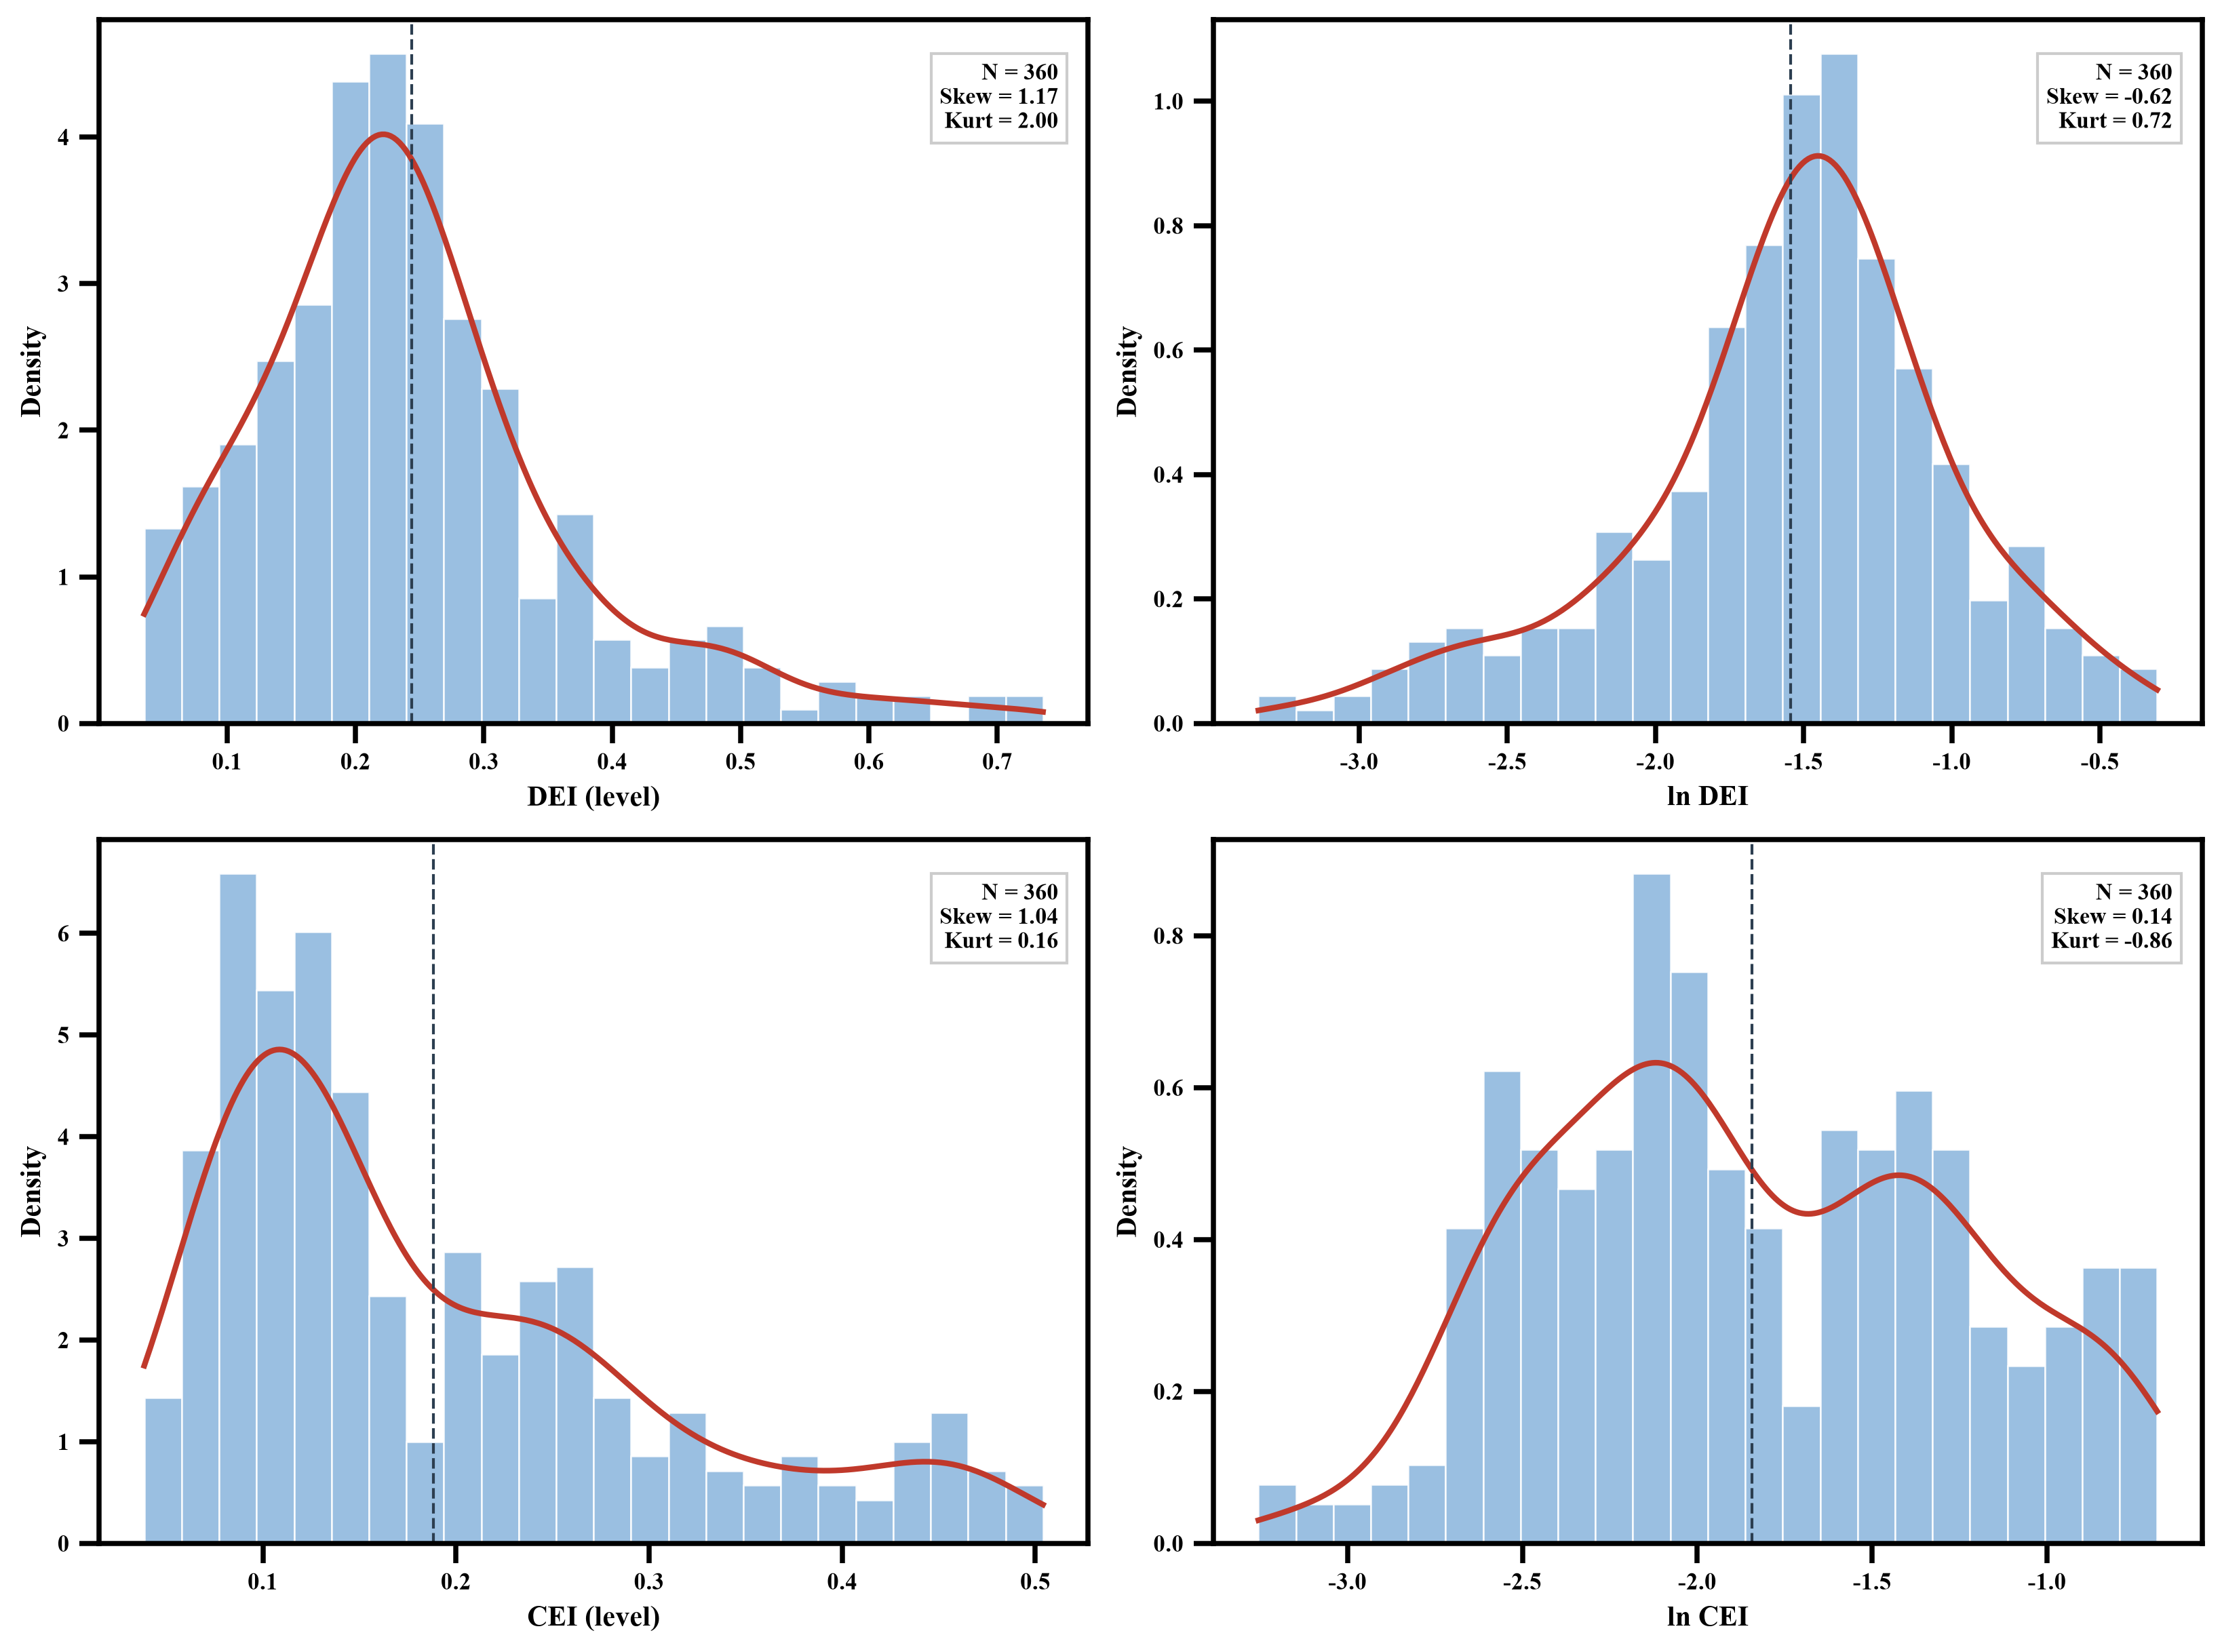
\includegraphics[width=\textwidth]{figures/fig03_distributions.png}
\caption{Distributions of the digital economy and carbon emission pressure indices before and after the log transformation ($N=360$). The histograms use 24 bins; the red curve is a Gaussian kernel density estimate; the dashed vertical line is the sample mean.}
\label{fig:dist}
\end{figure}

\subsection{PCA-Based Alternative Measures}

To test whether the results depend on the weighting scheme, we construct PCA-based alternatives. The KMO statistic is 0.8042 for the 13 digital economy indicators and 0.6532 for the four carbon indicators; the Bartlett tests reject the identity correlation matrix in both cases ($\chi^2=4875.590$, $df=78$, $p<0.001$ for DEI; $\chi^2=1103.777$, $df=6$, $p<0.001$ for CEI). We retain three principal components for the digital economy, which together explain 76.724\% of the variance, and one component for carbon pressure, which explains 66.574\% (Appendix Table \ref{tab:pca_eigen}).

The score of observation $i$ on component $k$ is
\begin{equation}
F_{ik}=\sum_j b_{jk}z_{ij},
\qquad
b_{jk}=\frac{v_{jk}}{\sqrt{\lambda_k}},
\label{eq:pca_score}
\end{equation}
where $z_{ij}$ is the standardized value of indicator $j$, $v_{jk}$ is the $k$-th eigenvector, and $\lambda_k$ is the corresponding eigenvalue. The composite score is
\begin{equation}
S_i=\sum_k \frac{\lambda_k}{\sum_l \lambda_l}F_{ik}.
\label{eq:pca_composite}
\end{equation}
To make the PCA estimates comparable to the baseline, we linearly map $S_i$ to the range of the combined-weight index:
\begin{equation}
\tilde S_i=S^{\min}_{\mathrm{base}}+\frac{S_i-S^{\min}}{S^{\max}-S^{\min}}
\left(S^{\max}_{\mathrm{base}}-S^{\min}_{\mathrm{base}}\right).
\label{eq:pca_map}
\end{equation}
The mapped index is positive and has the same range as the combined-weight index, so its log can enter the same log--log model. The PCA measures are robustness devices, not claims that PCA is a superior measurement model.

\subsection{Control Variables and Baseline Model}

The control set includes log per capita GDP ($\ln pgdp$), fiscal expenditure as a share of GDP ($fisc$), population density ($dens$), financial development ($fin$), urbanization ($urb$), and marketization ($mkt$). These variables capture the main competing explanations in the literature: the environmental Kuznets curve \citep{grossman1991,dietz1997}, fiscal capacity, land and population pressure, financial development, urbanization, and institutional development. Table \ref{tab:desc} reports definitions and descriptive statistics.

Two groups of variables are excluded from the baseline. Carbon intensity and its components are part of CEI, so including them would absorb variation in the outcome. Industrial structure ($inds$) and energy efficiency ($ee$) are mechanism variables; including them would control for the channel under test \citep{angrist2009,schisterman2009}. We therefore estimate the channels separately in Section 4.6.

\begin{table}[!htbp]
\centering
\caption{Variable definitions and descriptive statistics.}
\label{tab:desc}
\footnotesize
\setlength{\tabcolsep}{2.5pt}
\begin{threeparttable}
\begin{tabular}{llcccccc}
\toprule
Variable & Definition & $N$ & Mean & SD & Min & Max\\
\midrule
$DEI$ & Digital economy index (combined weight) & 360 & 0.2438 & 0.1241 & 0.0354 & 0.7355\\
$\ln DEI$ & Natural log of DEI & 360 & $-1.5446$ & 0.5435 & $-3.3404$ & $-0.3071$\\
$CEI$ & Carbon emission pressure index & 360 & 0.1882 & 0.1145 & 0.0386 & 0.5040\\
$\ln CEI$ & Natural log of CEI & 360 & $-1.8445$ & 0.5911 & $-3.2549$ & $-0.6852$\\
$\ln pgdp$ & Log per capita GDP & 360 & 10.8678 & 0.4610 & 9.6818 & 12.1547\\
$fisc$ & Fiscal expenditure/GDP & 360 & 0.2590 & 0.1115 & 0.1050 & 0.7583\\
$dens$ & Population density (people/km$^2$) & 360 & 471.1261 & 708.5574 & 7.8658 & 3951.4762\\
$fin$ & (Deposits + loans)/GDP & 360 & 3.4376 & 1.0848 & 1.6879 & 7.6178\\
$urb$ & Urbanization rate & 360 & 0.6014 & 0.1205 & 0.3503 & 0.8958\\
$mkt$ & Marketization index & 360 & 8.1497 & 1.9461 & 3.3590 & 12.8640\\
$inds$ & Industrial structure upgrading (tertiary/secondary) & 360 & 1.3572 & 0.7443 & 0.5271 & 5.2440\\
$ee$ & Energy efficiency (output per unit of energy) & 360 & 1.7700 & 0.8837 & 0.4568 & 6.0333\\
\bottomrule
\end{tabular}
\begin{tablenotes}\footnotesize
\item Notes: The sample is a balanced panel of 30 provinces from 2011 to 2022. $inds$ and $ee$ are mechanism variables and do not enter the baseline regression.
\end{tablenotes}
\end{threeparttable}
\end{table}

\subsection{Spatial Weight Matrices and Spatial Panel Models}

Spatial dependence can arise from two distinct structures. To separate them, we construct three baseline weight matrices and one composite matrix.

The geographic contiguity matrix $W^{\mathrm{adj}}$ uses Queen contiguity: $W_{ij}=1$ if provinces $i$ and $j$ share a border or a vertex, and zero otherwise. Hainan is treated as adjacent to Guangdong and Guangxi across the Qiongzhou Strait. The matrix has 132 directed nonzero entries (66 adjacent pairs), or about 4.4 neighbors per province.

The geographic distance matrix $W^{\mathrm{dist}}$ uses $W_{ij}=1/d_{ij}$ for $i\neq j$, where $d_{ij}$ is the great-circle distance between provincial capitals; each province is truncated to its five nearest neighbors and the matrix is row-standardized.

The economic distance matrix $W^{\mathrm{econ}}$ uses $W_{ij}=1/|\bar Y_i-\bar Y_j|$ for $i\neq j$, where $\bar Y_i$ is the sample-period average per capita GDP; each province is again truncated to its five nearest economic neighbors and row-standardized.

The composite matrix $W^{*}$ restricts neighbors to contiguous provinces but weights them by economic similarity:
\begin{equation}
W^{*}_{ij}=A_{ij}E_{ij},
\qquad
E_{ij}=\frac{1}{|\bar Y_i-\bar Y_j|}\;(i\neq j),
\qquad
W^{*}_{ii}=0,
\label{eq:composite_w}
\end{equation}
where $A_{ij}$ is the Queen contiguity indicator and the product is row-standardized. Geography defines who can be a neighbor; economic distance defines how much weight each neighbor receives.

Following \citet{lesage2009} and \citet{elhorst2014}, the spatial Durbin model (SDM) is
\begin{equation}
\begin{split}
\ln CEI_{it}={}&\rho\sum_{j=1}^{n}W_{ij}\ln CEI_{jt}
+\alpha\ln DEI_{it}
+\theta\sum_{j=1}^{n}W_{ij}\ln DEI_{jt}\\
&+\sum_k\gamma_k Control_{k,it}
+\sum_k\phi_k\sum_{j=1}^{n}W_{ij}Control_{k,jt}
+\mu_i+\tau_t+\varepsilon_{it}.
\end{split}
\label{eq:sdm}
\end{equation}
The spatial lag model (SAR) sets $\theta=\phi_k=0$:
\begin{equation}
\ln CEI_{it}=\rho\sum_{j=1}^{n}W_{ij}\ln CEI_{jt}
+\alpha\ln DEI_{it}+\sum_k\gamma_k Control_{k,it}
+\mu_i+\tau_t+\varepsilon_{it},
\label{eq:sar}
\end{equation}
and the spatial error model (SEM) places the spatial dependence in the error term:
\begin{equation}
\ln CEI_{it}=\alpha\ln DEI_{it}+\sum_k\gamma_k Control_{k,it}
+\mu_i+\tau_t+u_{it},
\qquad
u_{it}=\lambda\sum_{j=1}^{n}W_{ij}u_{jt}+\varepsilon_{it}.
\label{eq:sem}
\end{equation}
All three models are estimated by maximum likelihood with province and year fixed effects. For the SDM, the direct effect is the average effect of a province's own $\ln DEI$ on its own $\ln CEI$; the indirect effect is the average effect on other provinces; and the total effect is their sum. These are long-run effects because they incorporate the spatial multiplier $(I-\rho W)^{-1}$.

Global spatial autocorrelation is measured by Moran's $I$:
\begin{equation}
I=\frac{n\sum_{i=1}^{n}\sum_{j=1}^{n}w_{ij}(x_i-\bar x)(x_j-\bar x)}
{\sum_{i=1}^{n}\sum_{j=1}^{n}w_{ij}\sum_{i=1}^{n}(x_i-\bar x)^2},
\label{eq:moran}
\end{equation}
with inference based on the standardized $z$ statistic and, for robustness, 999 random permutations \citep{moran1950}. Local Moran statistics identify which provinces form high--high, low--high, high--low, and low--low clusters.

\subsection{Mechanism Tests}

We follow the two-step logic recommended by \citet{imai2010,bullock2010} and estimate two equations for each mechanism:
\begin{align}
\ln CEI_{it}&=c_0+c\ln DEI_{it}+\sum_k\gamma_k Control_{k,it}+\mu_i+\tau_t+\varepsilon_{it},
\label{eq:step1}\\
\ln M_{it}&=a_0+a\ln DEI_{it}+\sum_k\gamma_k Control_{k,it}+\mu_i+\tau_t+\varepsilon_{it},
\label{eq:step2}
\end{align}
where $M$ is industrial structure ($inds$) or energy efficiency ($ee$). Equation \eqref{eq:step1} is the baseline total association; Equation \eqref{eq:step2} is the first link of the channel. The second link---from $M$ to CEI---is supported by external evidence in Section 2. Both equations use the baseline controls and fixed effects.

\subsection{Dynamic Panel Specification}

Carbon pressure is persistent because energy infrastructure, capital stock, and consumption habits adjust slowly. We therefore estimate a system-GMM model:
\begin{equation}
\ln CEI_{it}=\rho\ln CEI_{i,t-1}+\beta\ln DEI_{it}
+\sum_k\gamma_k Control_{k,it}+\mu_i+\tau_t+\varepsilon_{it},
\label{eq:gmm}
\end{equation}
where $\rho$ measures persistence, $\beta$ is the short-run association, and the long-run association is $\beta/(1-\rho)$. We use the two-step estimator with Windmeijer-corrected standard errors \citep{windmeijer2005}. Instrument validity is assessed with the Hansen test, and residual serial correlation with AR(1) and AR(2) tests \citep{arellano1991,blundell1998,roodman2009}. The instrument count is kept below the number of provinces to avoid overfitting.

%=================================================================
\section{Results}

\subsection{Two Indices, Two Geographies}

The two composite indices tell a consistent measurement story before they enter any regression (Figure \ref{fig:maps}). The DEI rises from 0.09 in 2011 to 0.25 in 2016 and 0.35 in 2022, with Beijing, Guangdong, Shanghai, Jiangsu, and Zhejiang consistently at the top. The CEI falls from 0.219 in 2011 to 0.183 in 2016 and 0.169 in 2022, but the decline is uneven: Ningxia, Inner Mongolia, Xinjiang, and Qinghai remain in the highest-pressure class, while most southern provinces are in the lowest. The contrast is the empirical puzzle. If digital development and carbon pressure moved together, the map would show one gradient. Instead, it shows two: a digital gradient running from the coast to the interior, and a carbon gradient running from the northwest to the southeast. Beijing and Shanghai are both digital leaders, but Beijing sits in the lowest carbon-pressure class while Shanghai sits in the highest. The raw correlation between the two indices is therefore weak, and the conditional analysis is designed to ask whether the relationship emerges once income, industrial structure, energy endowments, and spatial dependence are accounted for.

\begin{figure}[!htbp]
\centering
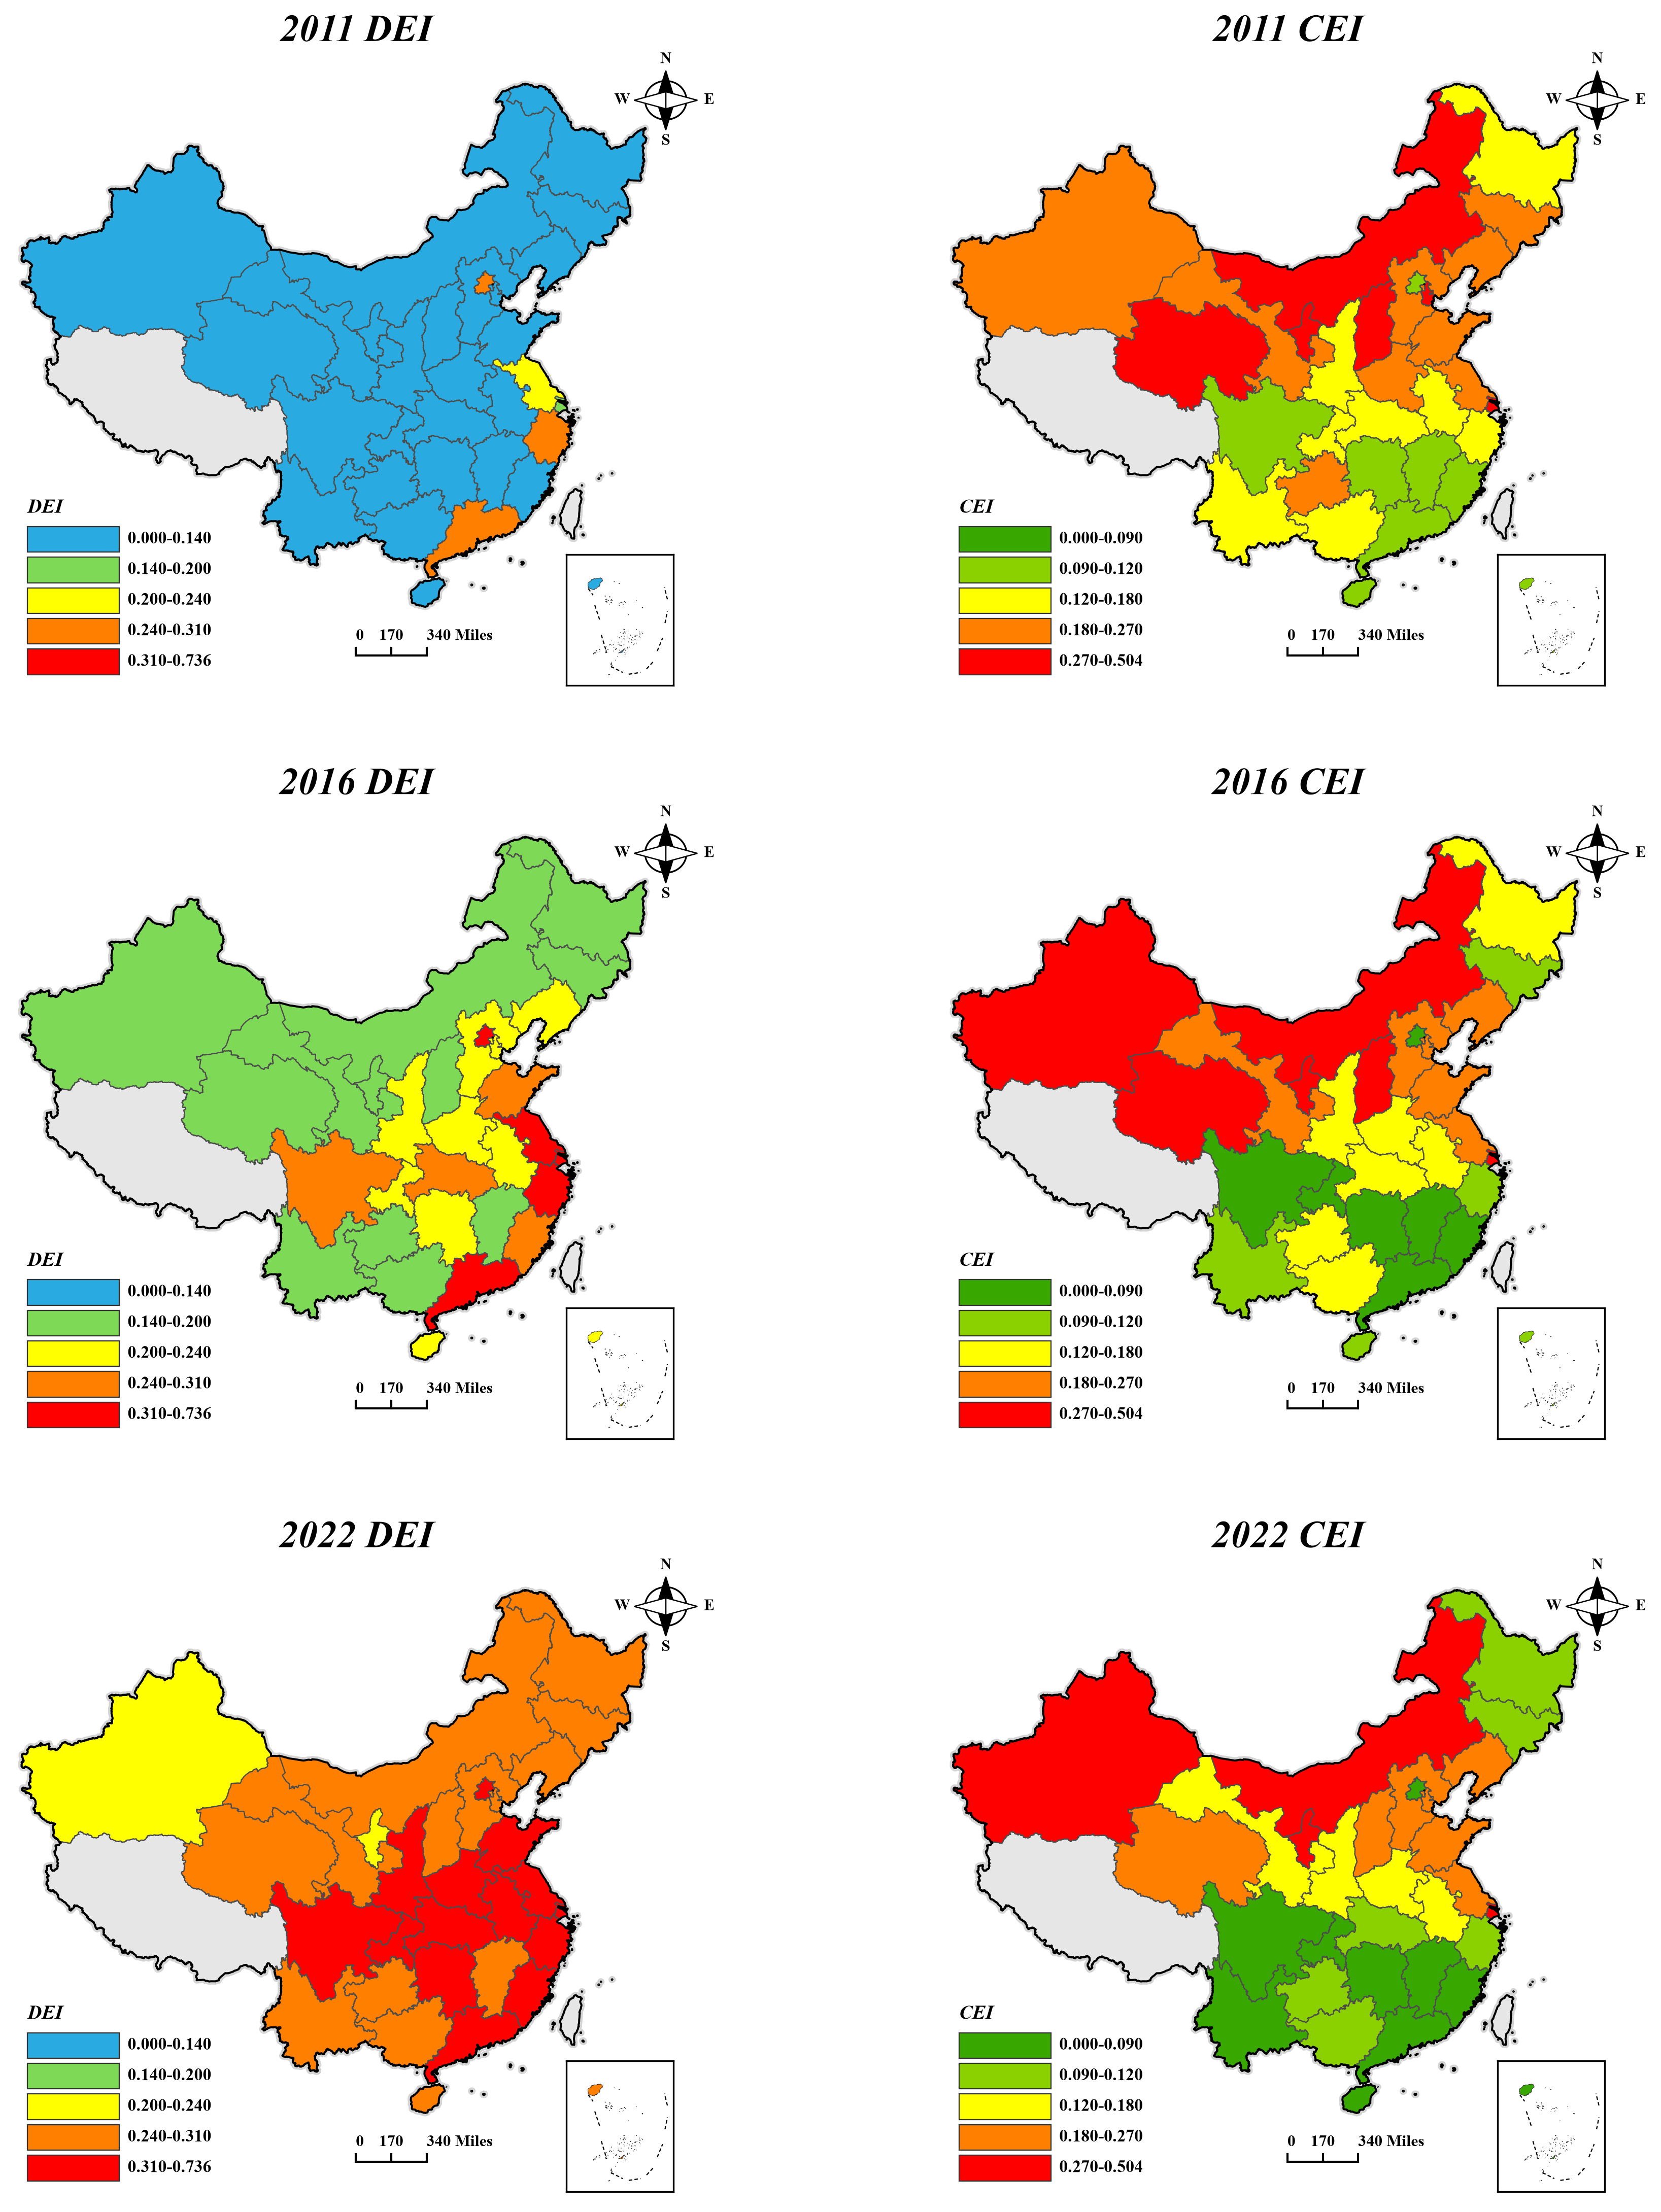
\includegraphics[width=\textwidth]{figures/fig02_maps.png}
\caption{Spatial distribution of the digital economy index (DEI) and carbon emission pressure index (CEI) in 2011, 2016, and 2022. The five classes use fixed breaks for each index, so colors are comparable across years. Tibet and Taiwan have no observations and are shown in gray; provincial boundaries are retained.}
\label{fig:maps}
\end{figure}

The weighting results support this reading. The combined weights are less concentrated than the entropy weights, and the PCA measures reproduce the main ranking but not every detail. The point is not that one weighting scheme is correct; it is that the substantive question should be answered with more than one measure. Table \ref{tab:dei} and Table \ref{tab:cei} report the indicator systems, and Table \ref{tab:desc} reports the descriptive statistics. The indices are right-skewed, which is why the analysis moves to logs.

\subsection{The Average Association}

Table \ref{tab:baseline} starts with pooled OLS without fixed effects (column 1, $-0.311$) and then adds province and year fixed effects and controls in pairs. With fixed effects and no controls, the elasticity is $-0.481$. Adding income and fiscal capacity moves it to $-0.338$; adding density and financial development moves it to $-0.280$; adding urbanization and marketization leaves it at $-0.278$. Most of the adjustment occurs at the first step, and the final estimate is stable. Read in proportional terms, a 10\% increase in DEI is associated with about a 2.8\% decrease in CEI. The elasticity is a proportional relationship: a province that moves from a low to a moderate digital level changes the percentage composition of its economy.

\begin{table}[!htbp]
\centering
\caption{Baseline estimates with controls added in pairs.}
\label{tab:baseline}
\footnotesize
\setlength{\tabcolsep}{6pt}
\begin{threeparttable}
\begin{tabular}{lccccc}
\toprule
 & (1) & (2) & (3) & (4) & (5)\\
\midrule
$\ln DEI$ & $-0.311^{**}$ & $-0.481^{***}$ & $-0.338^{***}$ & $-0.280^{***}$ & $-0.278^{***}$\\
 & (0.121) & (0.112) & (0.083) & (0.087) & (0.092)\\
$\ln pgdp$ & & & $-0.750^{***}$ & $-0.780^{***}$ & $-0.792^{***}$\\
 & & & (0.215) & (0.217) & (0.243)\\
$fisc$ & & & $-0.285$ & $-0.488$ & $-0.469$\\
 & & & (0.395) & (0.469) & (0.458)\\
$dens$ & & & & 0.001 & 0.001\\
 & & & & (0.001) & (0.001)\\
$fin$ & & & & 0.019 & 0.004\\
 & & & & (0.058) & (0.060)\\
$urb$ & & & & & $-0.471$\\
 & & & & & (0.716)\\
$mkt$ & & & & & 0.023\\
 & & & & & (0.022)\\
\midrule
Province FE & No & Yes & Yes & Yes & Yes\\
Year FE & No & Yes & Yes & Yes & Yes\\
Observations & 360 & 360 & 360 & 360 & 360\\
$R^2$ & 0.082 & 0.209 & 0.342 & 0.356 & 0.365\\
\bottomrule
\end{tabular}
\begin{tablenotes}\footnotesize
\item Notes: Standard errors in parentheses are clustered at the province level. $^{***}$, $^{**}$, and $^{*}$ denote significance at the 1\%, 5\%, and 10\% levels. Column (1) is pooled OLS without fixed effects and reports overall $R^2$. Columns (2)--(5) include province and year fixed effects and report within $R^2$; column (2) has no controls, column (3) adds $\ln pgdp$ and $fisc$, column (4) adds $dens$ and $fin$, and column (5) adds $urb$ and $mkt$. The baseline is column (5).
\end{tablenotes}
\end{threeparttable}
\end{table}


\subsection{Is the Result a Measurement Artifact?}

Table \ref{tab:pca_robust} reports the replacement estimates. We replace the outcome, the core regressor, and both with PCA-based measures. The elasticity remains negative in all three cases, and it remains significant at the 10\% level or better. The magnitude shrinks when both indices are replaced, which is exactly what classical measurement error predicts: PCA extracts common variation and discards indicator-specific variation, so the resulting measure is noisier and its coefficient is attenuated. The sign is the robust result; the magnitude depends on the measure.

\begin{table}[!htbp]
\centering
\caption{PCA-based measurement robustness.}
\label{tab:pca_robust}
\footnotesize
\setlength{\tabcolsep}{6pt}
\begin{threeparttable}
\begin{tabular}{lcccc}
\toprule
 & (1) Baseline & (2) PCA-CEI & (3) PCA-DEI & (4) Both PCA\\
\midrule
$\ln DEI$ & $-0.278^{***}$ & $-0.207^{***}$ & &\\
 & (0.092) & (0.061) & &\\
$\ln$ PCA-DEI & & & $-0.293^{*}$ & $-0.156^{*}$\\
 & & & (0.152) & (0.081)\\
\midrule
$\ln pgdp$ & $-0.792^{***}$ & $-0.527^{***}$ & $-0.772^{***}$ & $-0.563^{***}$\\
 & (0.243) & (0.141) & (0.237) & (0.143)\\
$fisc$ & $-0.469$ & 0.100 & $-0.421$ & 0.137\\
 & (0.458) & (0.283) & (0.462) & (0.287)\\
$dens$ & 0.0006 & $-0.0009^{*}$ & 0.0012$^{*}$ & $-0.0004$\\
 & (0.0006) & (0.0005) & (0.0006) & (0.0005)\\
$fin$ & 0.004 & $-0.043$ & 0.008 & $-0.049$\\
 & (0.060) & (0.040) & (0.063) & (0.040)\\
$urb$ & $-0.471$ & 0.924 & $-0.682$ & 0.763\\
 & (0.716) & (0.582) & (0.627) & (0.620)\\
$mkt$ & 0.023 & 0.008 & 0.028 & 0.010\\
 & (0.022) & (0.013) & (0.023) & (0.014)\\
\midrule
Outcome & $\ln CEI$ & $\ln$ PCA-CEI & $\ln CEI$ & $\ln$ PCA-CEI\\
Province FE & Yes & Yes & Yes & Yes\\
Year FE & Yes & Yes & Yes & Yes\\
Observations & 360 & 360 & 360 & 360\\
\bottomrule
\end{tabular}
\begin{tablenotes}\footnotesize
\item Notes: Standard errors clustered at the province level in parentheses. $^{***}$, $^{**}$, and $^{*}$ denote significance at the 1\%, 5\%, and 10\% levels. All columns include province and year fixed effects. Column (2) replaces the outcome with the PCA-based CEI; column (3) replaces the core regressor with the PCA-based DEI; column (4) replaces both.
\end{tablenotes}
\end{threeparttable}
\end{table}

\subsection{A Boundary Condition}

Table \ref{tab:extra_robust} reports the four checks. Lagging DEI by one year yields a negative and significant coefficient \citep{bellemare2017}. Excluding the four municipalities leaves the estimate essentially unchanged, and winsorizing at the 1st and 99th percentiles does the same. The pattern is stable across all three checks.

\begin{table}[!htbp]
\centering
\caption{Additional robustness checks.}
\label{tab:extra_robust}
\footnotesize
\setlength{\tabcolsep}{5pt}
\begin{threeparttable}
\begin{tabular}{lcccc}
\toprule
 & (1) Lagged & (2) Excl. & (3) Winsorized & (4) $\ln CE$\\
 & DEI & municipalities & 1\% & outcome\\
\midrule
$\ln DEI$ & $-0.303^{***}$ & $-0.276^{**}$ & $-0.286^{***}$ & $-0.009$\\
 & (0.079) & (0.110) & (0.104) & (0.063)\\
\midrule
$\ln pgdp$ & $-0.753^{***}$ & $-0.900^{***}$ & $-0.794^{***}$ & $-1.115^{***}$\\
 & (0.249) & (0.265) & (0.239) & (0.138)\\
$fisc$ & $-0.632$ & $-0.414$ & $-0.406$ & $-0.483$\\
 & (0.452) & (0.518) & (0.438) & (0.375)\\
$dens$ & 0.0007 & 0.0015 & 0.0007 & $-0.0012^{**}$\\
 & (0.0007) & (0.0011) & (0.0006) & (0.0006)\\
$fin$ & 0.025 & $-0.014$ & $-0.002$ & 0.003\\
 & (0.058) & (0.070) & (0.061) & (0.038)\\
$urb$ & $-0.364$ & 0.422 & $-0.342$ & 0.276\\
 & (0.705) & (1.255) & (0.734) & (0.467)\\
$mkt$ & 0.019 & 0.020 & 0.022 & 0.014\\
 & (0.020) & (0.021) & (0.022) & (0.017)\\
\midrule
Outcome & $\ln CEI$ & $\ln CEI$ & $\ln CEI$ & $\ln CE$\\
Province FE & Yes & Yes & Yes & Yes\\
Year FE & Yes & Yes & Yes & Yes\\
Observations & 330 & 312 & 360 & 360\\
\bottomrule
\end{tabular}
\begin{tablenotes}\footnotesize
\item Notes: Standard errors clustered at the province level in parentheses. $^{***}$, $^{**}$, and $^{*}$ denote significance at the 1\%, 5\%, and 10\% levels. All columns include province and year fixed effects. Column (1) lags DEI by one year; column (2) excludes Beijing, Shanghai, Tianjin, and Chongqing; column (3) winsorizes DEI and CEI at the 1st and 99th percentiles; column (4) uses log carbon intensity as the outcome.
\end{tablenotes}
\end{threeparttable}
\end{table}

The fourth check is different, and it is the most informative. When the outcome is carbon intensity alone, the coefficient is essentially zero. The composite pressure index aggregates intensity, per capita emissions, density, and energy intensity; the near-zero intensity result means that the negative composite association is not driven by lower carbon per unit of GDP. It is likely to reflect the per-capita, density, and energy-intensity components. The finding is about carbon emission pressure as a broad index, not about carbon intensity as a single indicator. The distinction matters for policy, because a strategy that targets digitalization alone may change the composition of activity without decarbonizing production at a given income level.

\subsection{Which Channel Matters?}

Table \ref{tab:mechanism} reports the two-step estimates. Energy efficiency carries the mechanism: DEI is positively associated with energy efficiency, and energy efficiency is negatively associated with carbon pressure; both links survive the controls and the two-way fixed effects. Industrial structure upgrading is positively associated with DEI, and its second link is supported by the evidence reviewed in Section 2. Energy efficiency is therefore the stronger of the two channels in this sample, consistent with recent evidence that digital development is associated with higher energy productivity and urban energy efficiency \citep{ma2024,wang2025energy}.

\begin{table}[!htbp]
\centering
\caption{Mechanism estimates: industrial structure and energy efficiency.}
\label{tab:mechanism}
\footnotesize
\setlength{\tabcolsep}{6pt}
\begin{threeparttable}
\begin{tabular}{lcccc}
\toprule
 & (1) & (2) & (3) & (4)\\
 & $\ln CEI$ & $\ln inds$ & $\ln ee$ & $\ln CEI$\\
\midrule
$\ln DEI$ & $-0.278^{***}$ & $0.247^{**}$ & $0.336^{**}$ & $-0.166^{*}$\\
 & (0.092) & (0.094) & (0.145) & (0.094)\\
$\ln ee$ & & & & $-0.335^{***}$\\
 & & & & (0.089)\\
\midrule
$\ln pgdp$ & $-0.792^{***}$ & $-0.478^{*}$ & $1.300^{***}$ & $-0.357$\\
 & (0.243) & (0.278) & (0.236) & (0.235)\\
$fisc$ & $-0.469$ & $1.507^{***}$ & $1.300^{***}$ & $-0.034$\\
 & (0.458) & (0.478) & (0.473) & (0.405)\\
$dens$ & 0.0006 & 0.0006 & 0.0024$^{***}$ & 0.0015$^{**}$\\
 & (0.0006) & (0.0008) & (0.0009) & (0.0007)\\
$fin$ & 0.004 & 0.064 & $-0.046$ & $-0.011$\\
 & (0.060) & (0.053) & (0.047) & (0.061)\\
$urb$ & $-0.471$ & 0.381 & $-0.955$ & $-0.790$\\
 & (0.716) & (0.675) & (1.035) & (0.679)\\
$mkt$ & 0.023 & $-0.014$ & 0.040 & 0.037$^{*}$\\
 & (0.022) & (0.017) & (0.027) & (0.020)\\
\midrule
Province FE & Yes & Yes & Yes & Yes\\
Year FE & Yes & Yes & Yes & Yes\\
Observations & 360 & 360 & 360 & 360\\
$R^2$ & 0.984 & 0.966 & 0.963 & 0.987\\
Adjusted $R^2$ & 0.981 & 0.961 & 0.958 & 0.985\\
\bottomrule
\end{tabular}
\begin{tablenotes}\footnotesize
\item Notes: Standard errors clustered at the province level in parentheses. $^{***}$, $^{**}$, and $^{*}$ denote significance at the 1\%, 5\%, and 10\% levels. Columns (1)--(3) form the two-step design \citep{imai2010,bullock2010}; column (4) estimates the second link, from energy efficiency to carbon pressure.
\end{tablenotes}
\end{threeparttable}
\end{table}


\subsection{Where Carbon Pressure Clusters}

Table \ref{tab:moran} reports the global Moran statistics. The spatial diagnostics reveal two different spatial processes. DEI is most strongly autocorrelated under the economic-distance weight, with Moran's $I$ around 0.49 and significance at the 1\% level in every year. Under geographic contiguity, the statistic is smaller and weakens over time. CEI shows the opposite pattern: it is positively and significantly autocorrelated under the two geographic weights, but negatively and insignificantly autocorrelated under economic distance. In other words, digital development clusters among economically similar provinces, while carbon pressure clusters among geographically adjacent provinces. The LISA maps tell the same story (Figure \ref{fig:localmoran}), and the main clusters persist across the three map years: Beijing, Shanghai, and Jiangsu form a high--high digital cluster, while Beijing is a low--high carbon outlier and Shanghai a high--low one; Ningxia sits inside the high--high carbon cluster.

\begin{table}[!htbp]
\centering
\caption{Global Moran's $I$ for DEI and CEI, selected years and period mean.}
\label{tab:moran}
\footnotesize
\setlength{\tabcolsep}{3.5pt}
\begin{threeparttable}
\begin{tabular}{lcccccc}
\toprule
 & \multicolumn{3}{c}{DEI} & \multicolumn{3}{c}{CEI}\\
\cmidrule(lr){2-4}\cmidrule(lr){5-7}
Year & Economic & Geographic & Contiguity & Economic & Geographic & Contiguity\\
 & distance & distance & & distance & distance & \\
\midrule
2011 & $0.589^{***}$ & $0.245^{***}$ & $0.248^{**}$ & $-0.218$ & $0.248^{***}$ & $0.308^{***}$\\
2016 & $0.489^{***}$ & 0.124 & $0.162^{*}$ & $-0.185$ & $0.295^{***}$ & $0.327^{***}$\\
2022 & $0.455^{***}$ & 0.090 & 0.100 & $-0.215$ & $0.248^{***}$ & $0.265^{***}$\\
Mean & $0.492^{***}$ & 0.146 & 0.174 & $-0.195$ & $0.273^{***}$ & $0.309^{***}$\\
\bottomrule
\end{tabular}
\begin{tablenotes}\footnotesize
\item Notes: $^{***}$, $^{**}$, and $^{*}$ denote significance at the 1\%, 5\%, and 10\% levels based on the two-sided $z$ test. The mean is the arithmetic average of the 12 annual estimates; its stars indicate the weakest significance level attained in all 12 years, not the significance of the average itself. Full annual series are plotted in Figure \ref{fig:moran}.
\end{tablenotes}
\end{threeparttable}
\end{table}
\begin{figure}[!htbp]
\centering
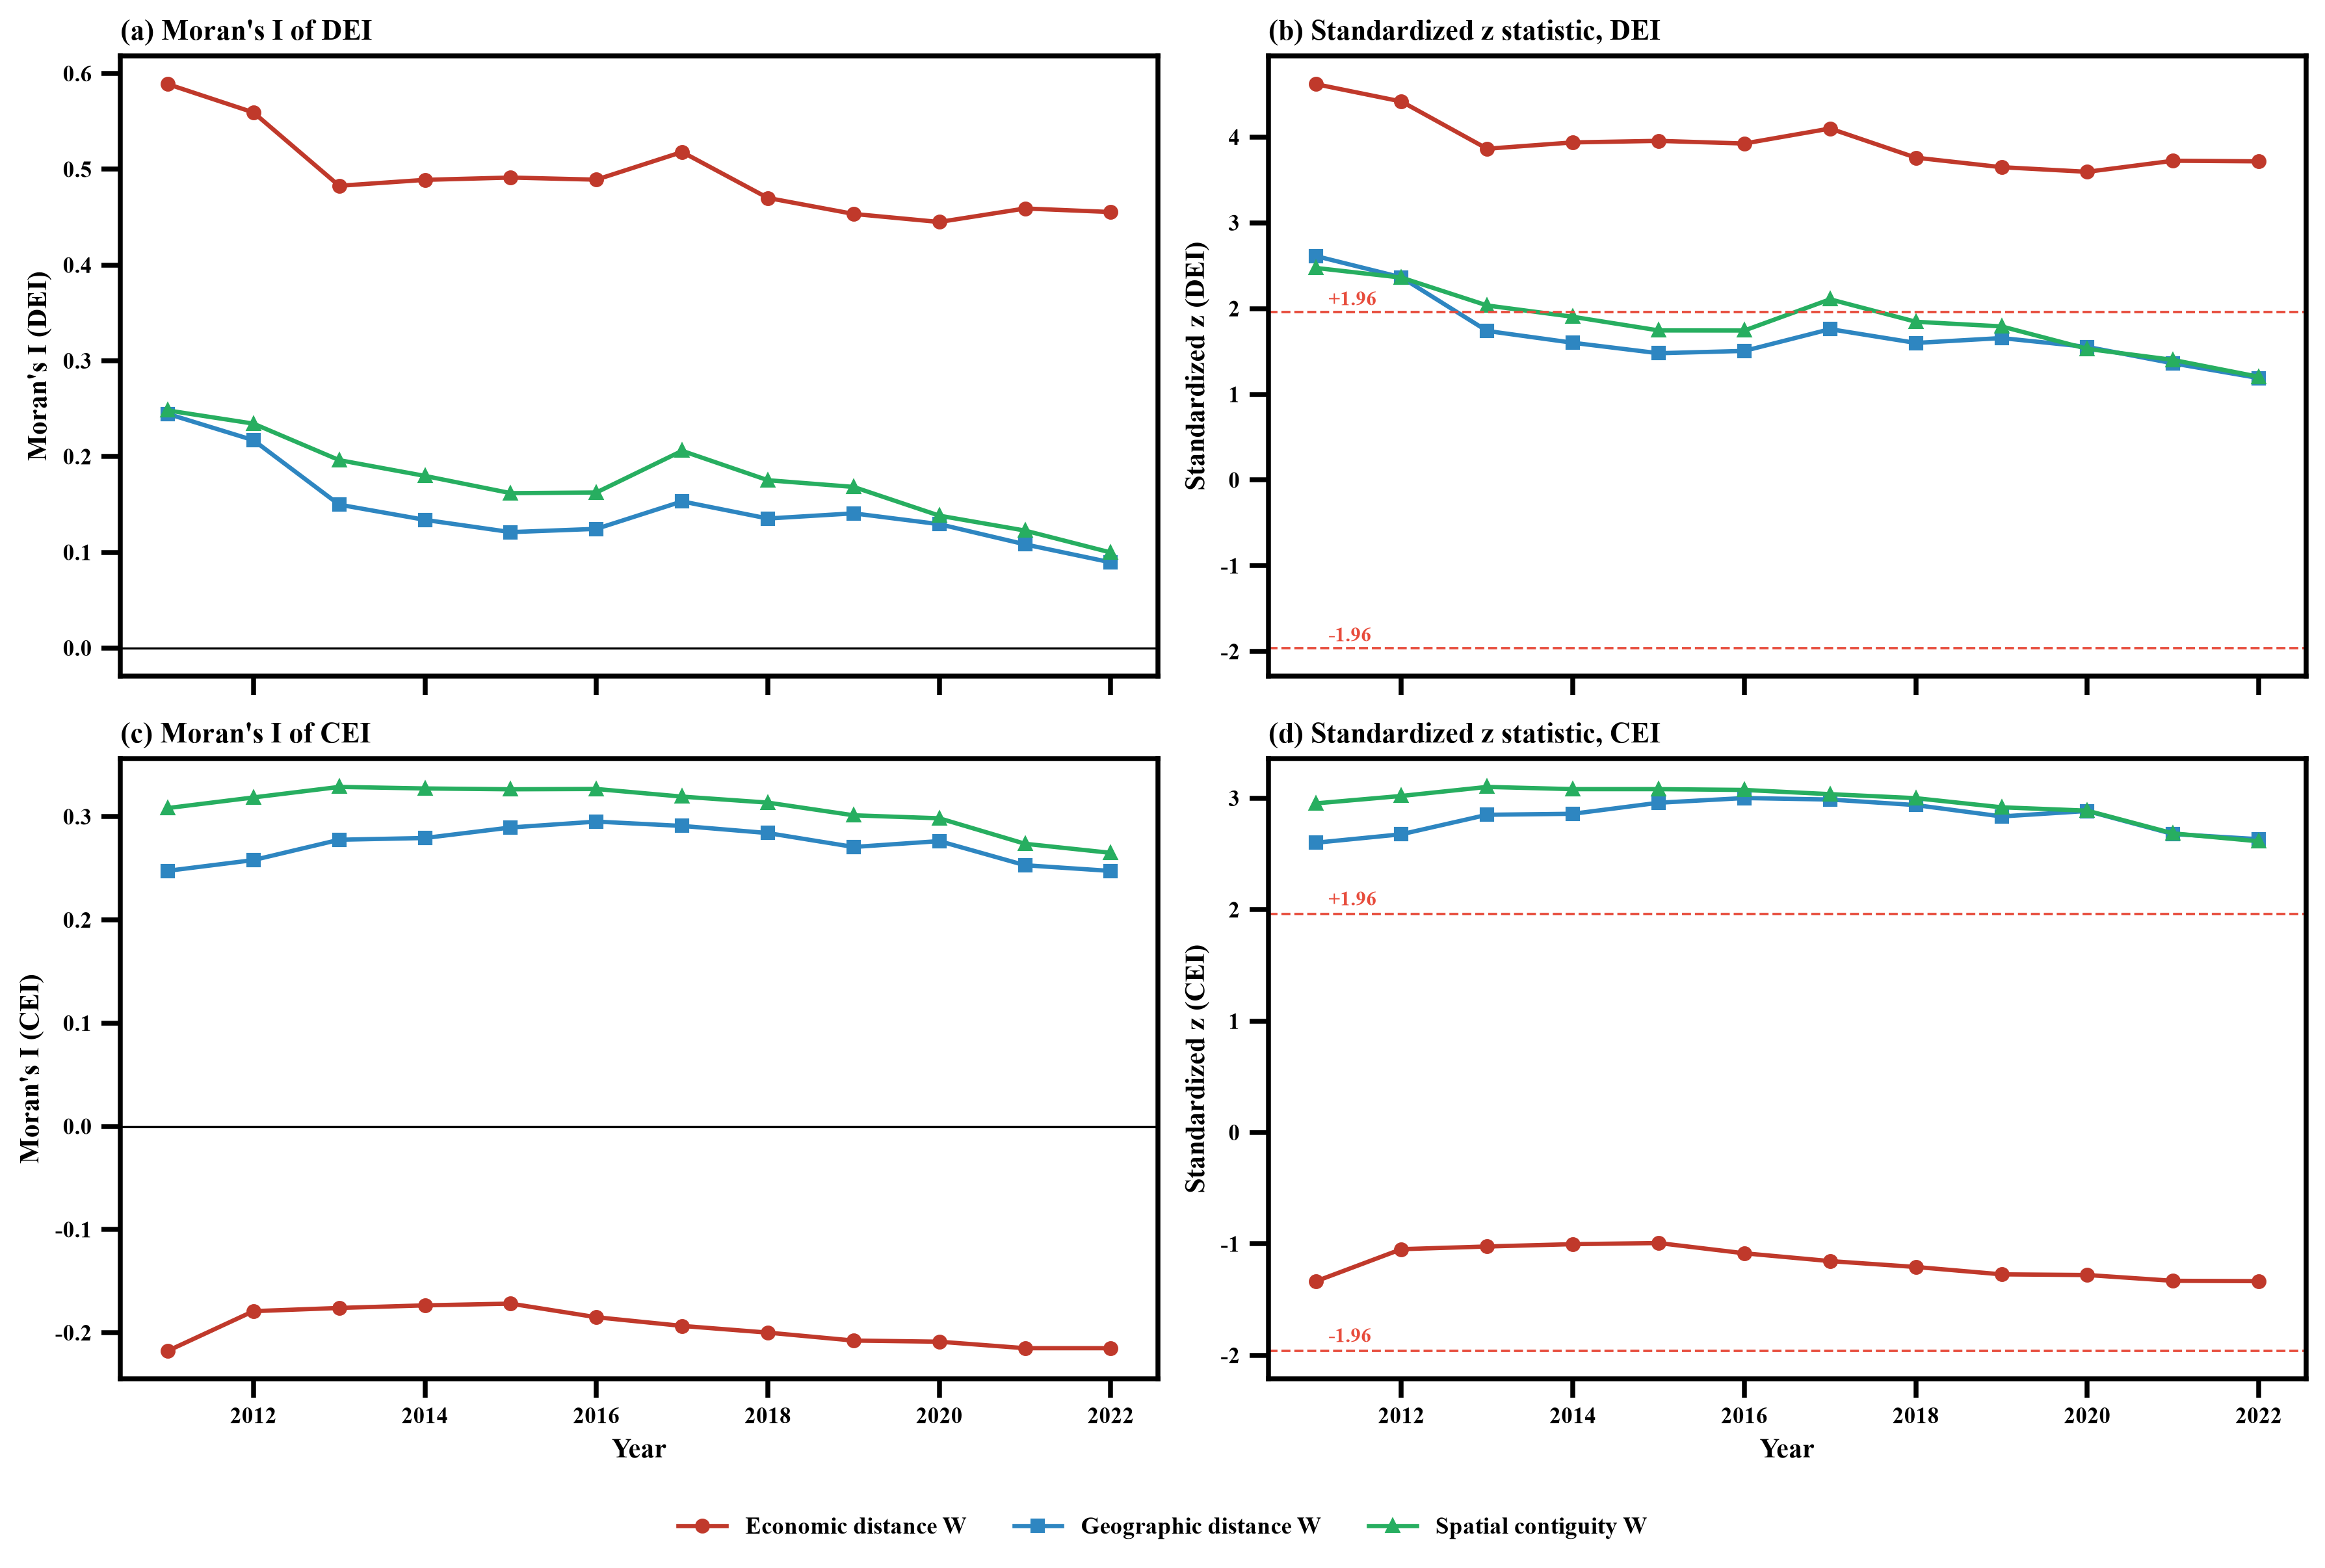
\includegraphics[width=\textwidth]{figures/fig04_moran.png}
\caption{Global Moran's $I$ and standardized $z$ statistics for DEI and CEI, 2011--2022, under three weight matrices. The dashed horizontal lines in panels (b) and (d) mark $\pm 1.96$.}
\label{fig:moran}
\end{figure}
\begin{figure}[!htbp]
\centering
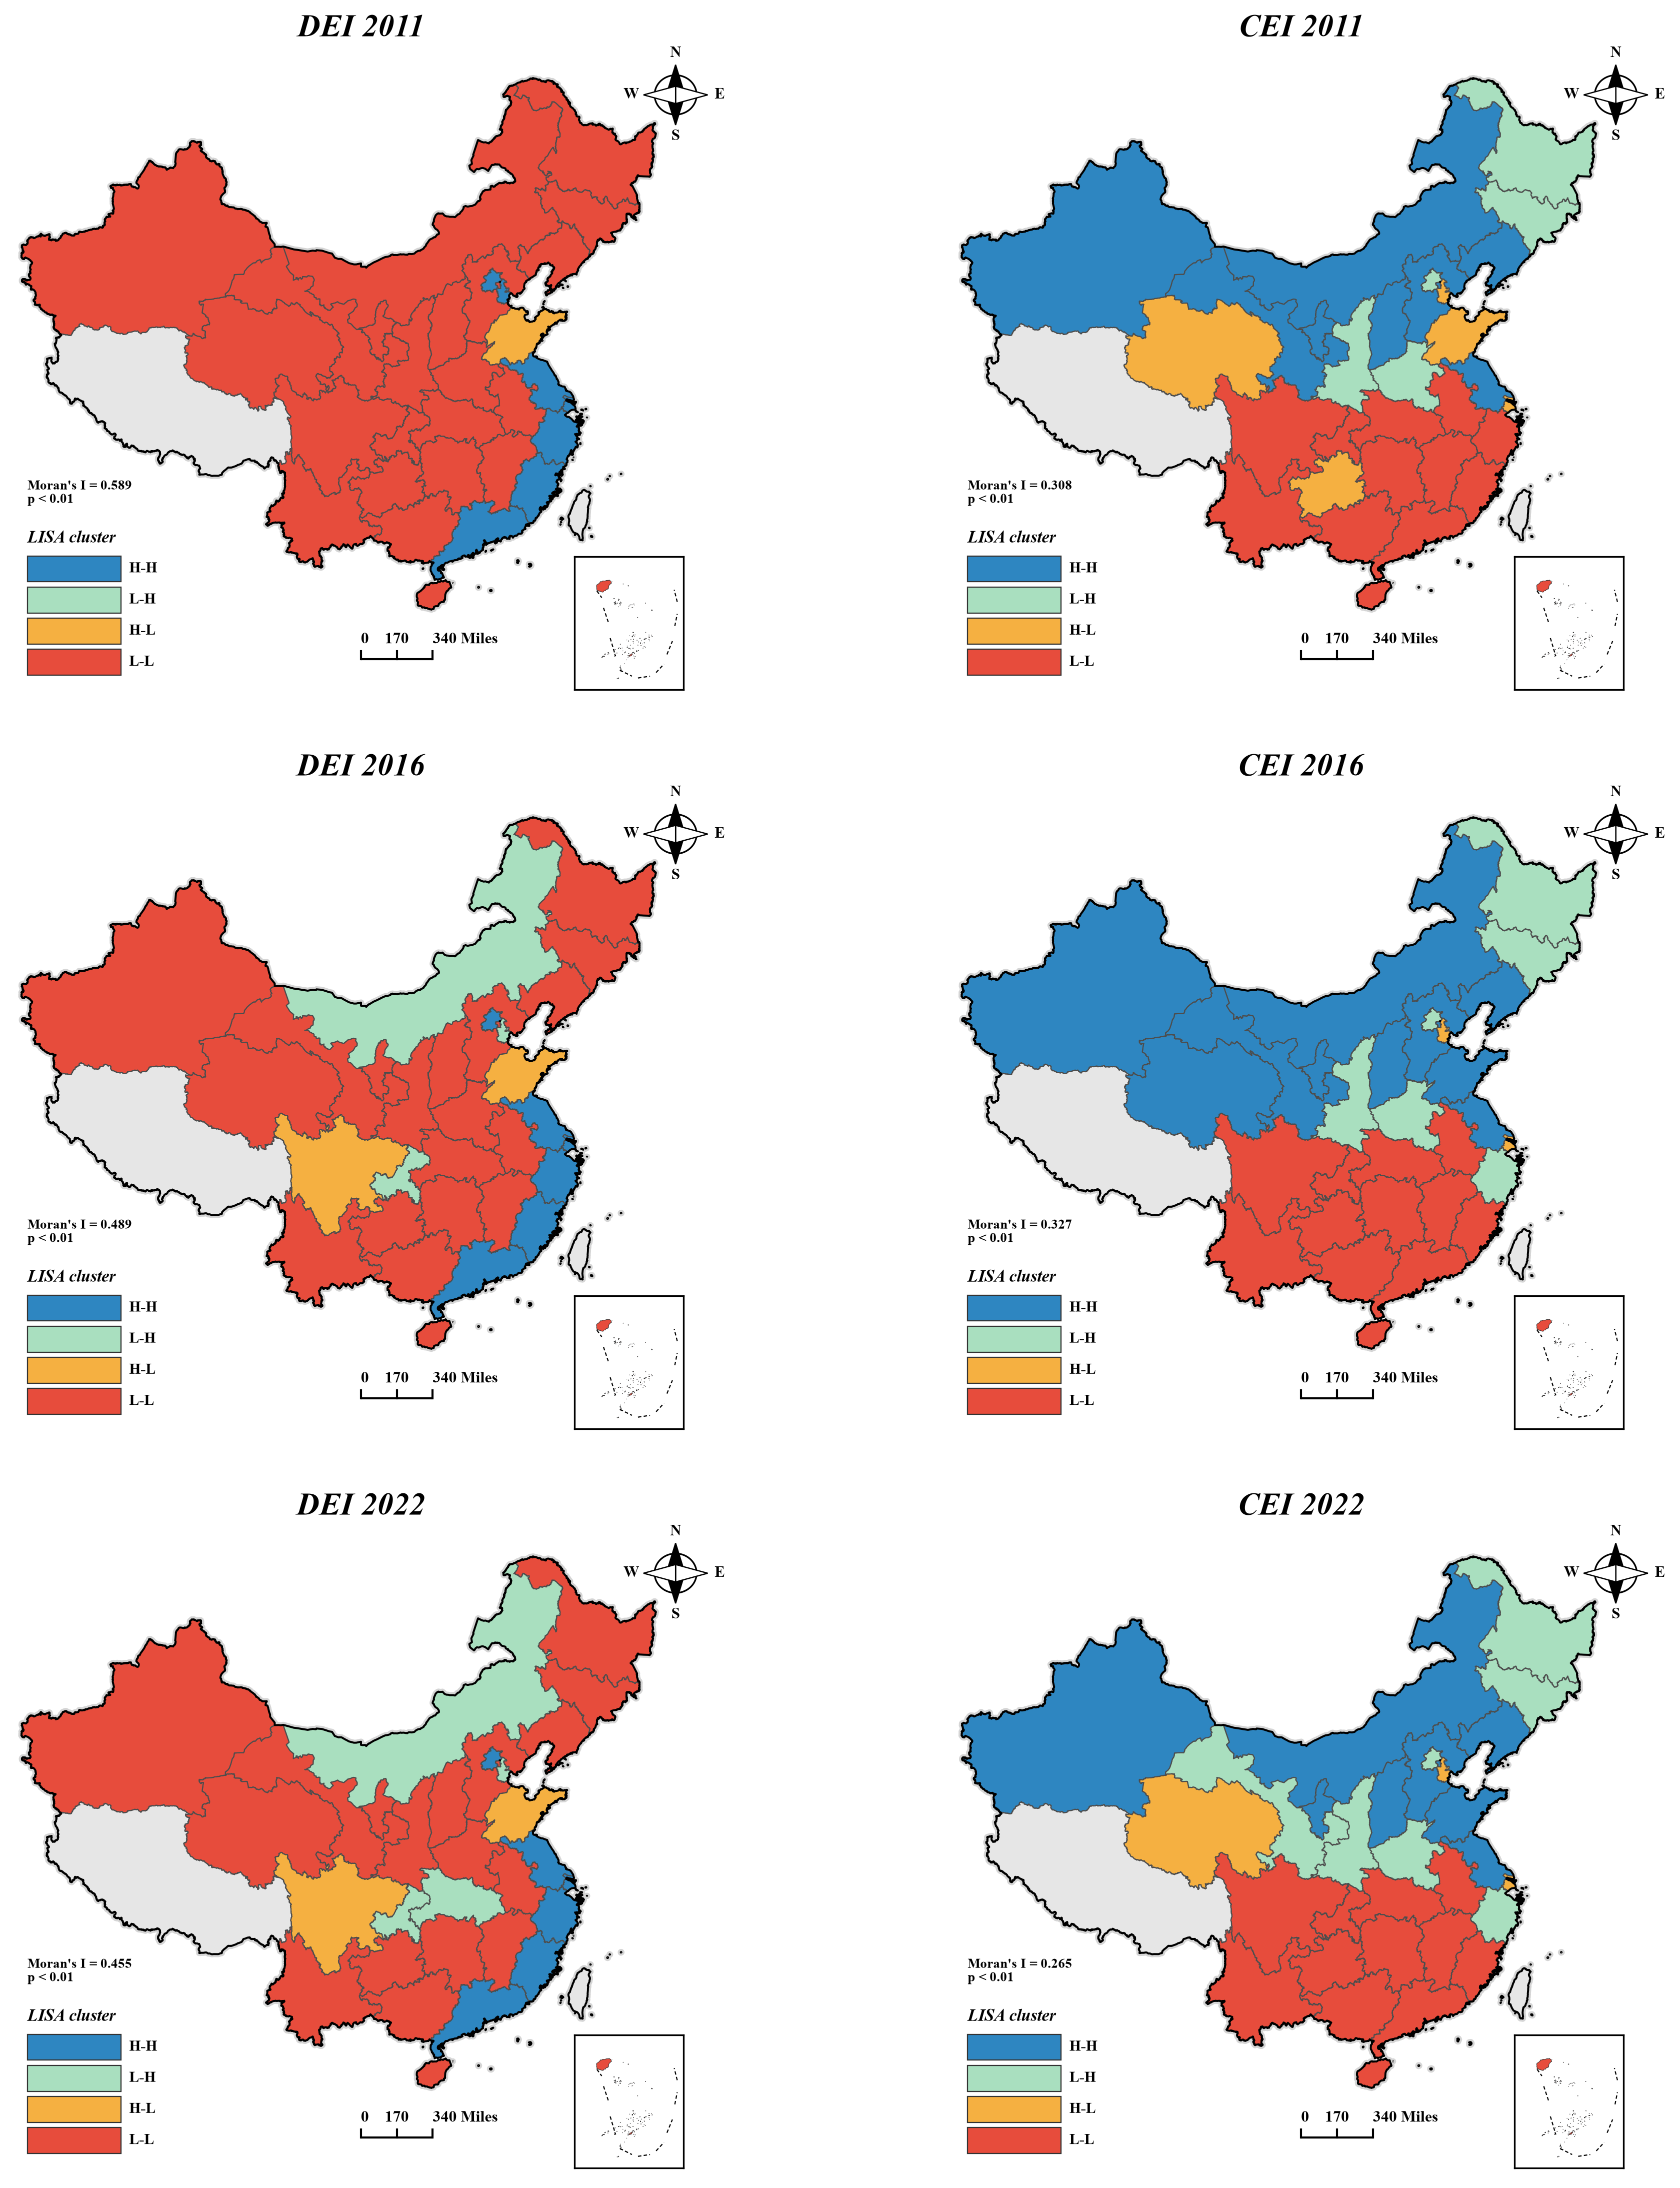
\includegraphics[width=\textwidth]{figures/fig05_lisa_maps.png}
\caption{Local Moran's $I$ quadrant maps for DEI (economic-distance weight) and CEI (contiguity weight) in 2011, 2016, and 2022. Colors indicate the H-H, L-H, H-L, and L-L quadrants. The statistics box reports global Moran's $I$ and its $p$-value. Tibet and Taiwan have no observations and are shown in grey.}
\label{fig:localmoran}
\end{figure}

\subsection{The Neighbor Definition Changes the Answer}

Table \ref{tab:spatial_composite} and Table \ref{tab:spatial_econ} report the spatial panel estimates. Under the composite weight, which restricts neighbors to contiguous provinces, the SDM direct effect is negative and significant, but the indirect effect is not. Under the pure economic-distance weight, the direct effect remains negative, and the indirect effect becomes negative and significant. The spatial autoregressive coefficient is large under the composite weight and essentially zero under the economic-distance weight, which makes the two results interpretable: the composite weight captures the geographic clustering of carbon pressure, while the economic-distance weight captures the diffusion of digital technology through industrial linkages. Spatial spillovers travel along economic linkages: digital development is associated with lower carbon pressure at home and in economically similar provinces, while administrative contiguity does not identify the indirect effect.

\begin{table}[H]
\centering
\caption{Spatial panel estimates under the composite contiguity--economic weight $W^{*}$.}
\label{tab:spatial_composite}
\scriptsize
\renewcommand{\arraystretch}{0.92}
\setlength{\tabcolsep}{4pt}
\begin{threeparttable}
\begin{tabular}{lccc}
\toprule
 & (1) & (2) & (3)\\
 & SDM & SAR & SEM\\
\midrule
\multicolumn{4}{l}{\textit{Main coefficients}}\\
$\ln DEI$ & $-0.194^{**}$ & $-0.223^{***}$ & $-0.242^{***}$\\
 & (0.090) & (0.075) & (0.086)\\
$\ln pgdp$ & $-0.877^{***}$ & $-0.802^{***}$ & $-0.820^{***}$\\
 & (0.207) & (0.213) & (0.200)\\
$fisc$ & $-0.474$ & $-0.425$ & $-0.405$\\
 & (0.305) & (0.407) & (0.495)\\
$dens$ & 0.000 & 0.001 & 0.000\\
 & (0.001) & (0.001) & (0.001)\\
$fin$ & 0.001 & $-0.009$ & $-0.007$\\
 & (0.043) & (0.054) & (0.058)\\
$urb$ & $-0.771$ & $-0.253$ & $-0.637$\\
 & (0.561) & (0.666) & (0.673)\\
$mkt$ & 0.018 & 0.023 & 0.019\\
 & (0.016) & (0.020) & (0.020)\\
\midrule
\multicolumn{4}{l}{\textit{Spatial lags of explanatory variables (SDM only)}}\\
$W^{*}\ln DEI$ & $-0.048$ & --- & ---\\
 & (0.104) & & \\
$W^{*}\ln pgdp$ & 0.196 & --- & ---\\
 & (0.262) & & \\
$W^{*}fisc$ & $-0.307$ & --- & ---\\
 & (1.367) & & \\
$W^{*}dens$ & 0.001 & --- & ---\\
 & (0.001) & & \\
$W^{*}fin$ & 0.046 & --- & ---\\
 & (0.058) & & \\
$W^{*}urb$ & 1.643 & --- & ---\\
 & (1.158) & & \\
$W^{*}mkt$ & 0.024 & --- & ---\\
 & (0.026) & & \\
\midrule
\multicolumn{4}{l}{\textit{Long-run effects of $\ln DEI$}}\\
Direct & $-0.206^{**}$ & $-0.227^{***}$ & ---\\
 & (0.096) & (0.080) & \\
Indirect & $-0.156$ & $-0.076^{*}$ & ---\\
 & (0.151) & (0.043) & \\
Total & $-0.362^{*}$ & $-0.303^{***}$ & ---\\
 & (0.203) & (0.111) & \\
\midrule
$\rho$ / $\lambda$ & $0.332^{***}$ & $0.264^{***}$ & $0.326^{***}$\\
 & (0.073) & (0.088) & (0.078)\\
Log-likelihood & 438.770 & 428.140 & 429.528\\
Within $R^2$ & 0.750 & 0.738 & 0.739\\
Observations & 360 & 360 & 360\\
\bottomrule
\end{tabular}
\begin{tablenotes}\footnotesize
\item Notes: Robust standard errors in parentheses. $^{***}$, $^{**}$, and $^{*}$ denote significance at the 1\%, 5\%, and 10\% levels. All models include province and year fixed effects and the six controls. The weight is $W^{*}=A\odot E$, where $A$ is Queen contiguity and $E$ is the inverse economic distance; the product is row-standardized. The lower block reports long-run effects. The SEM does not provide an effect decomposition.
\end{tablenotes}
\end{threeparttable}
\end{table}
\begin{table}[H]
\centering
\caption{Spatial Durbin estimates under the pure economic-distance weight.}
\label{tab:spatial_econ}
\scriptsize
\renewcommand{\arraystretch}{0.92}
\setlength{\tabcolsep}{4pt}
\begin{threeparttable}
\begin{tabular*}{0.62\textwidth}{@{\extracolsep{\fill}}lc}
\toprule
 & (1)\\
 & SDM\\
\midrule
\multicolumn{2}{l}{\textit{Main coefficients}}\\
$\ln DEI$ & $-0.407^{***}$\\
 & (0.113)\\
$\ln pgdp$ & $-0.866^{***}$\\
 & (0.208)\\
$fisc$ & $-0.445$\\
 & (0.422)\\
$dens$ & 0.001\\
 & (0.001)\\
$fin$ & 0.001\\
 & (0.056)\\
$urb$ & 0.735\\
 & (0.743)\\
$mkt$ & 0.025\\
 & (0.019)\\
\midrule
\multicolumn{2}{l}{\textit{Spatial lags of explanatory variables}}\\
$W^{\mathrm{econ}}\ln DEI$ & $-0.347^{**}$\\
 & (0.131)\\
$W^{\mathrm{econ}}\ln pgdp$ & 0.160\\
 & (0.457)\\
$W^{\mathrm{econ}}fisc$ & $-0.698$\\
 & (0.673)\\
$W^{\mathrm{econ}}dens$ & 0.002\\
 & (0.001)\\
$W^{\mathrm{econ}}fin$ & 0.105\\
 & (0.086)\\
$W^{\mathrm{econ}}urb$ & $5.691^{***}$\\
 & (1.625)\\
$W^{\mathrm{econ}}mkt$ & $-0.060$\\
 & (0.057)\\
\midrule
\multicolumn{2}{l}{\textit{Long-run effects of $\ln DEI$}}\\
Direct & $-0.403^{***}$\\
 & (0.116)\\
Indirect & $-0.364^{**}$\\
 & (0.186)\\
Total & $-0.767^{***}$\\
 & (0.272)\\
\midrule
$\rho$ & 0.012\\
 & (0.103)\\
Log-likelihood & 445.513\\
Within $R^2$ & 0.777\\
Observations & 360\\
\bottomrule
\end{tabular*}
\begin{tablenotes}\footnotesize
\item Notes: Robust standard errors in parentheses. $^{***}$, $^{**}$, and $^{*}$ denote significance at the 1\%, 5\%, and 10\% levels. The weight is the pure economic-distance matrix (inverse absolute difference in average per capita GDP, five nearest neighbors, row-standardized). All models include province and year fixed effects and the six controls. The likelihood-ratio tests reject the SAR ($LR=37.96$, $df=7$, $p<0.001$) and the SEM ($LR=27.55$, $df=7$, $p<0.001$).
\end{tablenotes}
\end{threeparttable}
\end{table}

\subsection{A Strong West, But No Formal Regional Difference}

Table \ref{tab:region} reports the interaction and subsample estimates. Regional heterogeneity is limited in the interaction model but visible in the subsample estimates. The interaction model does not reject homogeneity: the central and western interaction terms are small and insignificant. The subsample model tells a different descriptive story: the western elasticity is $-0.688$ and significant, while the eastern and central estimates are not. The two exercises answer different questions. The interaction model asks whether the regional difference is statistically significant under common slopes; the subsample model asks how strong the within-region association is. The western result is a direction for policy.

\begin{table}[H]
\centering
\caption{Regional heterogeneity: interaction and subsample estimates.}
\label{tab:region}
\footnotesize
\setlength{\tabcolsep}{4pt}
\begin{threeparttable}
\begin{tabular}{lccccc}
\toprule
 & (1) & (2) & (3) & (4) & (5)\\
 & Baseline & Interaction & East & Central & West\\
\midrule
$\ln DEI$ & $-0.278^{***}$ & $-0.235$ & $-0.024$ & $-0.261$ & $-0.688^{**}$\\
 & (0.092) & (0.153) & (0.127) & (0.194) & (0.267)\\
$\ln DEI\times$ central & & $-0.050$ & & & \\
 & & (0.071) & & & \\
$\ln DEI\times$ west & & $-0.010$ & & & \\
 & & (0.085) & & & \\
\midrule
$\ln pgdp$ & $-0.792^{***}$ & $-0.775^{***}$ & $-0.392$ & $-0.283$ & $-1.109^{**}$\\
 & (0.243) & (0.248) & (0.280) & (0.423) & (0.475)\\
$fisc$ & $-0.469$ & $-0.332$ & $-0.795$ & 0.317 & $-1.016$\\
 & (0.458) & (0.597) & (0.569) & (1.194) & (0.983)\\
$dens$ & 0.0006 & 0.0005 & 0.0007$^{**}$ & 0.0078 & 0.0046\\
 & (0.0006) & (0.0005) & (0.0003) & (0.0050) & (0.0044)\\
$fin$ & 0.004 & 0.003 & 0.051 & 0.070 & 0.098\\
 & (0.060) & (0.060) & (0.046) & (0.114) & (0.066)\\
$urb$ & $-0.471$ & $-0.489$ & $-0.215$ & $-1.230$ & $-3.834$\\
 & (0.716) & (0.759) & (0.855) & (2.745) & (3.523)\\
$mkt$ & 0.023 & 0.023 & 0.022 & 0.014 & 0.035\\
 & (0.022) & (0.020) & (0.024) & (0.037) & (0.047)\\
\midrule
Province FE & Yes & Yes & Yes & Yes & Yes\\
Year FE & Yes & Yes & Yes & Yes & Yes\\
Observations & 360 & 360 & 132 & 96 & 132\\
$R^2$ & 0.984 & 0.984 & 0.995 & 0.983 & 0.984\\
\bottomrule
\end{tabular}
\begin{tablenotes}\footnotesize
\item Notes: Standard errors clustered at the province level in parentheses. $^{***}$, $^{**}$, and $^{*}$ denote significance at the 1\%, 5\%, and 10\% levels. Columns (1)--(2) center $\ln DEI$ at the full-sample mean; province fixed effects absorb the region main effects. Columns (3)--(5) estimate separate subsample models and allow all coefficients and year effects to differ across regions. Coefficients in columns (3)--(5) are not directly comparable to the interaction coefficients in column (2).
\end{tablenotes}
\end{threeparttable}
\end{table}
\begin{figure}[!htbp]
\centering
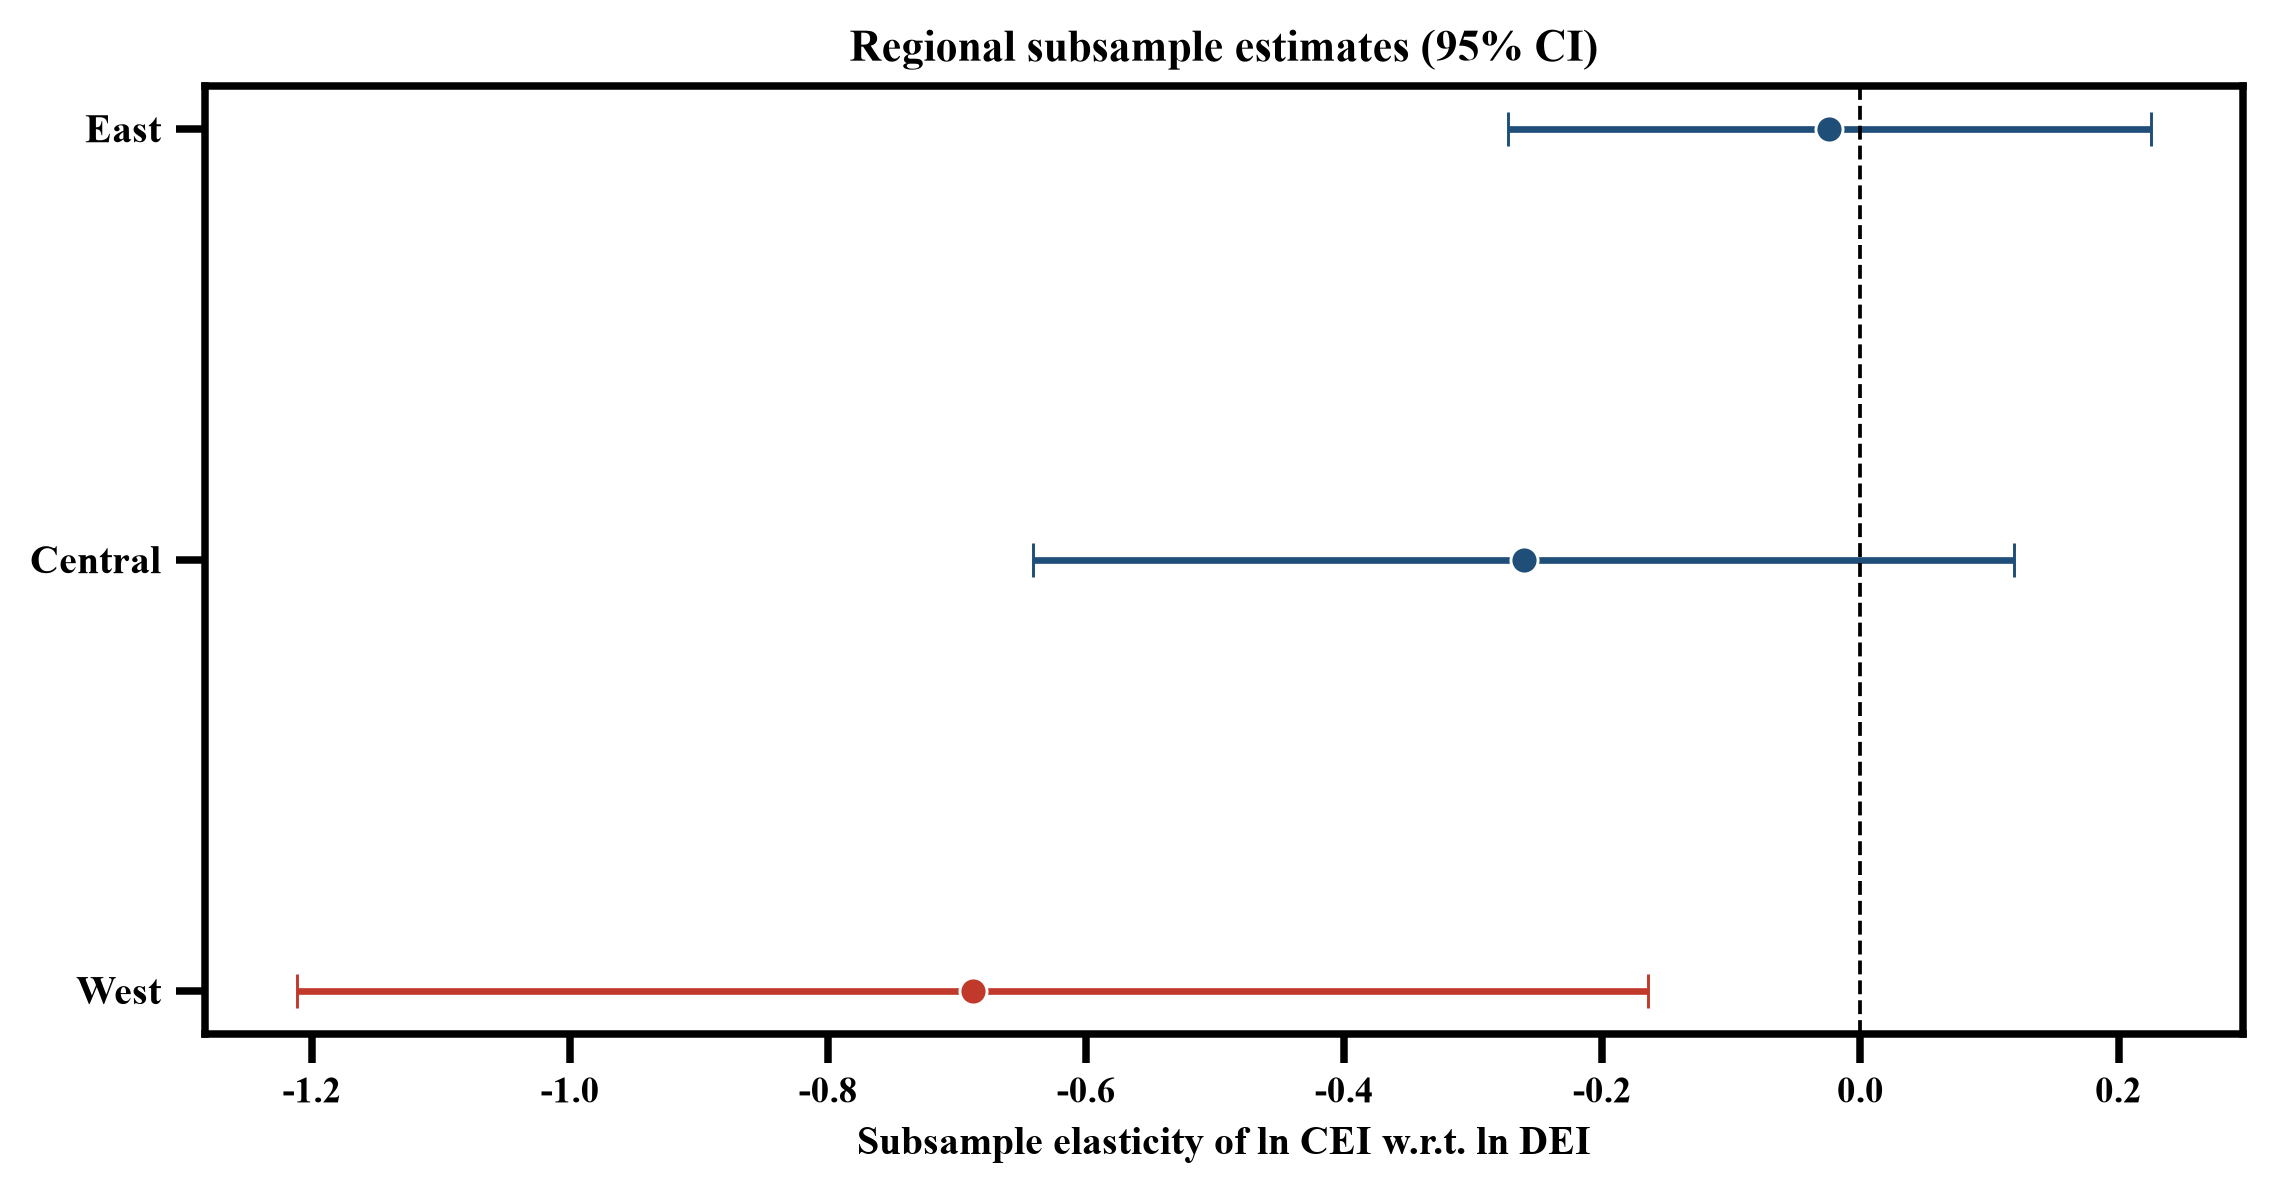
\includegraphics[width=0.72\textwidth]{figures/fig06_regional.png}
\caption{Subsample elasticities of carbon emission pressure with respect to the digital economy, by region, with 95\% confidence intervals. The interaction model in Table \ref{tab:region} does not reject regional homogeneity; the western subsample estimate is descriptive.}
\label{fig:regional}
\end{figure}

\subsection{Persistence Without Identification}

Table \ref{tab:gmm} reports the dynamic panel estimates. The dynamic panel confirms that carbon pressure is persistent: the coefficient on lagged CEI is 0.919. That is economically sensible, because energy infrastructure and capital stock adjust slowly. The short-run DEI coefficient is not significant. The dynamic specification is therefore informative about persistence, not about short-run digitalization. The static two-way fixed-effects estimate remains the main result.

\begin{table}[H]
\centering
\caption{System-GMM estimates of the dynamic relationship.}
\label{tab:gmm}
\footnotesize
\setlength{\tabcolsep}{4pt}
\begin{threeparttable}
\begin{tabular*}{0.75\textwidth}{@{\extracolsep{\fill}}lcc}
\toprule
 & (1) Current effect & (2) With lagged $\ln DEI$\\
\midrule
$L.\ln CEI$ & $0.919^{***}$ & $0.579^{*}$\\
 & (0.244) & (0.313)\\
$\ln DEI$ & $-0.119$ & $-0.660$\\
 & (0.354) & (0.748)\\
$L.\ln DEI$ & & 0.534\\
 & & (0.377)\\
\midrule
$\ln pgdp$ & $-0.101$ & $-1.964^{*}$\\
 & (0.993) & (1.180)\\
$fisc$ & 0.660 & 0.116\\
 & (0.709) & (0.918)\\
$dens$ & 0.0005 & 0.0028\\
 & (0.0012) & (0.0019)\\
$fin$ & $-0.009$ & $-0.313$\\
 & (0.143) & (0.217)\\
$urb$ & $-0.626$ & $-2.815$\\
 & (2.229) & (4.488)\\
$mkt$ & 0.006 & 0.068\\
 & (0.033) & (0.047)\\
\midrule
Province FE & Yes & Yes\\
Year FE & Yes & Yes\\
Observations & 330 & 330\\
Instruments & 22 & 23\\
AR(1) $p$ value & 0.009 & 0.732\\
AR(2) $p$ value & 0.066 & 0.463\\
Hansen $p$ value & 0.128 & 0.374\\
\bottomrule
\end{tabular*}
\begin{tablenotes}\footnotesize
\item Notes: Two-step system GMM with Windmeijer-corrected standard errors in parentheses. $^{***}$, $^{**}$, and $^{*}$ denote significance at the 1\%, 5\%, and 10\% levels. The dependent variable is $\ln CEI$. Province fixed effects are removed by the difference/orthogonal-deviation transformation; year dummies are treated as strictly exogenous. $\ln CEI$ and $\ln DEI$ (and $L.\ln DEI$ in column (2)) are treated as endogenous and instrumented with second and deeper lags, with collapse. Column (1) implies a long-run association of $-1.463$, which is reported for reference only because it has no standard error.
\end{tablenotes}
\end{threeparttable}
\end{table}

\section{Discussion}

\subsection{Main Findings and Recent Evidence}

The baseline elasticity is $-0.278$: a 10\% increase in DEI is associated with about a 2.8\% decrease in CEI. This is consistent with recent provincial evidence that digital development reduces carbon emissions or carbon intensity \citep{gao2024,huangwu2024,song2024,zhang2024sust,zhang2025}. The magnitude reflects the composite pressure outcome, the two-way fixed-effects design, and the broad DEI measure. The result is also consistent with the spatial studies that find negative spillovers from digital development to neighboring emissions \citep{yuan2024,wang2025,niu2024}.

The component-level check sharpens the interpretation. The near-zero estimate for carbon intensity alone means that the negative composite association is not driven by lower carbon per unit of GDP. It is likely to reflect the per-capita, density, and energy-intensity components. The finding is therefore about carbon emission pressure as a broad index, not about carbon intensity as a single indicator. This distinction should be kept in policy discussions: digitalization may change the composition and spatial organization of activity without decarbonizing production at a given income level.

\subsection{Measurement, Functional Form, and Mechanisms}

Composite indices are bounded, right-skewed, and often dominated by a few leading provinces. In levels, the coefficient is a semi-elasticity that depends on index units and is sensitive to the right tail; in logs, it is an elasticity that uses proportional variation. The log specification follows directly from the distribution of these indices, and the elasticity remains stable as controls are added in pairs.

The PCA results add a second measurement lesson. The negative association survives all three replacement strategies, but the magnitude is attenuated when both indices are replaced. This is the expected pattern under classical measurement error: PCA extracts common variation and discards indicator-specific variation, so the resulting measure is noisier and its coefficient is attenuated toward zero. The sign is robust; the magnitude depends on the measure.

The mechanism results point to energy efficiency. Energy efficiency is supported at both links: DEI is positively associated with energy efficiency, and energy efficiency is negatively associated with carbon pressure. Industrial structure upgrading is positively associated with DEI at the first link, and its second link is supported by the evidence reviewed in Section 2. This is consistent with recent evidence that digital development is associated with higher energy productivity and urban energy efficiency \citep{ma2024,wang2025energy}. The policy implication is to prioritize digital energy management over digital service expansion per se: industrial internet platforms, smart grids, and energy-management systems can reduce energy input per unit of output, while service expansion alone may not.

\subsection{Neighbor Definition and Policy Implications}

The spatial results show that the spillover conclusion depends on the neighbor definition. Under the composite weight, which restricts neighbors to contiguous provinces, the indirect effect is insignificant. Under the pure economic-distance weight, the indirect effect is $-0.364$ and significant. The most plausible interpretation is that digital technology diffuses through industrial chains, investment, and trade rather than across administrative borders. This is consistent with the negative spillovers reported by \citet{yuan2024} and the spatial dependence documented by \citet{wang2025} and \citet{niu2024}.

The policy implications follow. First, digital infrastructure investment should be paired with green-computing standards, because data centers and networks are energy-intensive. Second, energy-efficiency retrofits in energy-intensive industries should be the priority; the energy-efficiency channel is the stronger of the two mechanisms in our sample. Third, regional targeting should prioritize the west for digital infrastructure and energy-efficiency retrofits, but industrial transfer should be conditional on energy-efficiency and carbon-intensity thresholds. Fourth, measurement policy should report both composite and intensity measures, because they can lead to different conclusions.

\subsection{Scope and Future Work}

The design covers 30 provinces over 12 years and links digital development to carbon pressure through measurement, mechanism, and spatial channels. Policy shocks such as the Broadband China pilot \citep{xiao2024,lim2025} offer a natural next step for identification, and firm-level data would help distinguish technology diffusion from reallocation. Alternative proximity measures, such as input--output linkages or migration networks, would also enrich the spatial analysis. These extensions build on the measurement and neighbor-definition results developed here.

\section{Conclusions}

This study examines the relationship between the digital economy and carbon emission pressure in 30 Chinese provinces from 2011 to 2022. We construct a DEI from 13 indicators and a CEI from four indicators, combine entropy and CRITIC--Spearman weights, and cross-validate the results with PCA measures. Because both indices are right-skewed, we estimate log--log two-way fixed-effects models, supplemented by spatial Durbin models and system GMM.

Three findings stand out. First, the baseline elasticity is $-0.278$ ($p<0.01$): a 1\% increase in DEI is associated with a 0.278\% decrease in CEI, and a 10\% increase with about a 2.8\% decrease. The negative association survives PCA replacement, lagged DEI, exclusion of municipalities, and winsorization, but the magnitude is attenuated when both indices are replaced by PCA measures. Second, energy efficiency is the stronger mechanism: DEI is positively associated with energy efficiency, and energy efficiency is negatively associated with carbon pressure. Industrial structure upgrading is positively associated with DEI and operates at the first link. Third, spatial spillovers depend on the neighbor definition: they are negative and significant under economic distance and not under administrative contiguity.

The policy implications follow. Digitalization should be treated as a complement to, not a substitute for, energy-efficiency and carbon-pricing policies. Green-computing standards, energy-management systems, and industrial internet platforms are more likely to deliver a net reduction than digital service expansion alone. Regional policy should prioritize the west for digital infrastructure and energy-efficiency retrofits, but it should attach carbon-intensity thresholds to industrial transfer. Measurement policy should report both composite and intensity measures, because they can lead to different conclusions. Future research can use policy shocks, firm-level data, and alternative proximity measures to strengthen identification and distinguish technology diffusion from pollution-haven reallocation.

%=================================================================
\authorcontributions{Conceptualization, M.F. and Y.W.; methodology, M.F.; software, M.F.; validation, Y.W.; formal analysis, M.F.; data curation, M.F.; writing---original draft preparation, M.F.; writing---review and editing, Y.W.; visualization, M.F.; supervision, Y.W. All authors have read and agreed to the published version of the manuscript.}

\funding{This research received no external funding.}

\institutionalreview{Not applicable.}

\informedconsent{Not applicable.}

\dataavailability{The data used in this study are compiled from public statistical yearbooks, the China Internet Network Information Center, the Ministry of Industry and Information Technology, and the Peking University Digital Financial Inclusion Index. The processed panel, spatial weight matrices, replication code, and the manuscript source are openly available at \url{https://github.com/KarlHeinrich-jpg/digital-economy-carbon-emissions-china}.}

\conflictsofinterest{The authors declare no conflicts of interest.}

%=================================================================
\appendixstart
\appendix
\section{PCA Details}

Table \ref{tab:pca_eigen} reports the eigenvalues and variance contributions of the principal components, and Table \ref{tab:pca_load} reports the unrotated loadings used to construct the PCA measures.

\begin{table}[H]
\centering
\caption{PCA eigenvalues and variance contributions.}
\label{tab:pca_eigen}
\small
\begin{threeparttable}
\begin{tabular}{lcccc}
\toprule
\multicolumn{5}{l}{\textit{Digital economy (13 indicators)}}\\
Component & Eigenvalue & Variance (\%) & Cumulative (\%) & Retained\\
\midrule
F1 & 6.5178 & 50.137 & 50.137 & Yes\\
F2 & 2.2742 & 17.493 & 67.631 & Yes\\
F3 & 1.1821 & 9.093 & 76.724 & Yes\\
F4 & 0.8868 & 6.822 & 83.545 & No\\
\midrule
\multicolumn{5}{l}{\textit{Carbon emission pressure (4 indicators)}}\\
Component & Eigenvalue & Variance (\%) & Cumulative (\%) & Retained\\
\midrule
G1 & 2.6630 & 66.574 & 66.574 & Yes\\
G2 & 0.9753 & 24.383 & 90.957 & No\\
G3 & 0.3043 & 7.608 & 98.566 & No\\
G4 & 0.0574 & 1.434 & 100.000 & No\\
\bottomrule
\end{tabular}
\begin{tablenotes}\footnotesize
\item Notes: The Kaiser criterion (eigenvalue $>1$) is used to select components. Loadings are unrotated. The KMO statistics are 0.8042 for the digital economy indicators and 0.6532 for the carbon indicators; both Bartlett tests reject the identity matrix at $p<0.001$.
\end{tablenotes}
\end{threeparttable}
\end{table}

\begin{table}[H]
\centering
\caption{PCA loading matrix.}
\label{tab:pca_load}
\small
\begin{threeparttable}
\begin{tabular}{lccc}
\toprule
\multicolumn{4}{l}{\textit{Digital economy indicators}}\\
Indicator & PC1 & PC2 & PC3\\
\midrule
$X_1$ Domain names & 0.724 & 0.313 & 0.035\\
$X_2$ IPv4 addresses & 0.603 & 0.475 & $-0.378$\\
$X_3$ Internet access ports & 0.713 & 0.029 & 0.600\\
$X_4$ Mobile phone penetration & 0.793 & $-0.075$ & $-0.403$\\
$X_5$ Optical cable density & 0.611 & 0.049 & $-0.281$\\
$X_6$ Informatization enterprises & 0.600 & 0.446 & 0.565\\
$X_7$ Websites per 100 enterprises & 0.262 & 0.596 & $-0.223$\\
$X_8$ E-commerce transaction value & 0.872 & 0.291 & 0.040\\
$X_9$ Share of enterprises with e-commerce & 0.767 & $-0.235$ & $-0.236$\\
$X_{10}$ Software business revenue & 0.845 & 0.370 & 0.058\\
$X_{11}$ Coverage breadth & 0.771 & $-0.613$ & 0.012\\
$X_{12}$ Usage depth & 0.808 & $-0.521$ & 0.039\\
$X_{13}$ Digitization level & 0.618 & $-0.681$ & 0.066\\
\midrule
\multicolumn{4}{l}{\textit{Carbon emission indicators}}\\
Indicator & PC1 & & \\
\midrule
$Y_1$ Carbon emission intensity & 0.972 & & \\
$Y_2$ Per capita carbon emissions & 0.830 & & \\
$Y_3$ Carbon emission density & $-0.361$ & & \\
$Y_4$ Energy consumption intensity & 0.948 & & \\
\bottomrule
\end{tabular}
\begin{tablenotes}\footnotesize
\item Notes: Unrotated loadings. The carbon loadings have been sign-aligned so that the composite score moves in the same direction as carbon intensity.
\end{tablenotes}
\end{threeparttable}
\end{table}

%=================================================================
\clearpage
\reftitle{References}
\begin{thebibliography}{99}

\bibitem[\protect\citeauthoryear{Angrist \BBA\ Pischke}{{2009}}]{angrist2009}
Angrist, J. D., \& Pischke, J.-S. (2009). \textit{Mostly harmless econometrics: An empiricist's companion}. Princeton University Press.

\bibitem[\protect\citeauthoryear{Arellano \BBA\ Bond}{{1991}}]{arellano1991}
Arellano, M., \& Bond, S. (1991). Some tests of specification for panel data: Monte Carlo evidence and an application to employment equations. \textit{The Review of Economic Studies}, \textit{58}(2), 277--297. \url{https://doi.org/10.2307/2297968}

\bibitem[\protect\citeauthoryear{Bellemare et al.}{{2017}}]{bellemare2017}
Bellemare, M. F., Masaki, T., \& Pepinsky, T. B. (2017). Lagged explanatory variables and the estimation of causal effect. \textit{The Journal of Politics}, \textit{79}(3), 949--963. \url{https://doi.org/10.1086/690946}

\bibitem[\protect\citeauthoryear{Blundell \BBA\ Bond}{{1998}}]{blundell1998}
Blundell, R., \& Bond, S. (1998). Initial conditions and moment restrictions in dynamic panel data models. \textit{Journal of Econometrics}, \textit{87}(1), 115--143. \url{https://doi.org/10.1016/S0304-4076(98)00009-8}

\bibitem[\protect\citeauthoryear{Bullock et al.}{{2010}}]{bullock2010}
Bullock, J. G., Green, D. P., \& Ha, S. E. (2010). Yes, but what's the mechanism? (Don't expect an easy answer). \textit{Journal of Personality and Social Psychology}, \textit{98}(4), 550--558. \url{https://doi.org/10.1037/a0018933}

\bibitem[\protect\citeauthoryear{Diakoulaki et al.}{{1995}}]{diakoulaki1995}
Diakoulaki, D., Mavrotas, G., \& Papayannakis, L. (1995). Determining objective weights in multiple criteria problems: The CRITIC method. \textit{Computers \& Operations Research}, \textit{22}(7), 763--770. \url{https://doi.org/10.1016/0305-0548(94)00059-H}

\bibitem[\protect\citeauthoryear{Dietz \BBA\ Rosa}{{1997}}]{dietz1997}
Dietz, T., \& Rosa, E. A. (1997). Effects of population and affluence on CO$_2$ emissions. \textit{Proceedings of the National Academy of Sciences}, \textit{94}(1), 175--179. \url{https://doi.org/10.1073/pnas.94.1.175}

\bibitem[\protect\citeauthoryear{Elhorst}{{2014}}]{elhorst2014}
Elhorst, J. P. (2014). \textit{Spatial econometrics: From cross-sectional data to spatial panels}. Springer.

\bibitem[\protect\citeauthoryear{G20}{{2016}}]{g20}
G20. (2016). \textit{G20 digital economy development and cooperation initiative}. G20 Hangzhou Summit.

\bibitem[\protect\citeauthoryear{Gao et al.}{{2024}}]{gao2024}
Gao, J., Zhou, W., Cheng, J., \& Liu, Z. (2024). Digital economy development, common prosperity, and carbon emissions: An empirical study in China. \textit{Economies}, \textit{12}(5), Article 120. \url{https://doi.org/10.3390/economies12050120}

\bibitem[\protect\citeauthoryear{Gillingham \BBA\ Rapson}{{2016}}]{gillingham2016}
Gillingham, K., \& Rapson, D. (2016). The rebound effect and energy efficiency policy. \textit{Review of Environmental Economics and Policy}, \textit{10}(1), 68--88. \url{https://doi.org/10.1093/reep/rev017}

\bibitem[\protect\citeauthoryear{Goldfarb \BBA\ Tucker}{{2019}}]{goldfarb2019}
Goldfarb, A., \& Tucker, C. (2019). Digital economics. \textit{Journal of Economic Literature}, \textit{57}(1), 3--43. \url{https://doi.org/10.1257/jel.20171452}

\bibitem[\protect\citeauthoryear{Grossman \BBA\ Krueger}{{1991}}]{grossman1991}
Grossman, G. M., \& Krueger, A. B. (1991). \textit{Environmental impacts of a North American free trade agreement} (NBER Working Paper No. 3914). National Bureau of Economic Research. \url{https://doi.org/10.3386/w3914}

\bibitem[\protect\citeauthoryear{Guo et al.}{{2020}}]{guo2020report}
Guo, F., Wang, J., Wang, F., Kong, T., Zhang, X., \& Cheng, Z. (2020). \textit{The Peking University Digital Financial Inclusion Index of China}. Institute of Digital Finance, Peking University.

\bibitem[\protect\citeauthoryear{Huang \BBA\ Wu}{{2024}}]{huangwu2024}
Huang, F., \& Wu, C. (2024). Impact of digital economy on carbon emissions and its mechanism: Evidence from China. \textit{Sustainability}, \textit{16}(20), Article 8926. \url{https://doi.org/10.3390/su16208926}

\bibitem[\protect\citeauthoryear{Imai et al.}{{2010}}]{imai2010}
Imai, K., Keele, L., \& Tingley, D. (2010). A general approach to causal mediation analysis. \textit{Psychological Methods}, \textit{15}(4), 309--334. \url{https://doi.org/10.1037/a0020761}

\bibitem[\protect\citeauthoryear{IPCC}{{2006}}]{ipcc2006}
Intergovernmental Panel on Climate Change. (2006). \textit{2006 IPCC guidelines for national greenhouse gas inventories}. IGES.

\bibitem[\protect\citeauthoryear{LeSage \BBA\ Pace}{{2009}}]{lesage2009}
LeSage, J., \& Pace, R. K. (2009). \textit{Introduction to spatial econometrics}. CRC Press.

\bibitem[\protect\citeauthoryear{Li et al.}{{2025}}]{lim2025}
Li, M., Liang, S., Cheng, C., \& Du, W. (2025). Digital infrastructure investment and carbon emissions reduction based on the Broadband China policy. \textit{Utilities Policy}, \textit{95}, Article 101964. \url{https://doi.org/10.1016/j.jup.2025.101964}

\bibitem[\protect\citeauthoryear{Liu \BBA\ Wang}{{2025}}]{liuwang2025}
Liu, B., \& Wang, F. (2025). The impact of the global digital economy on carbon emissions: A review. \textit{Sustainability}, \textit{17}(11), Article 5044. \url{https://doi.org/10.3390/su17115044}

\bibitem[\protect\citeauthoryear{Ma et al.}{{2024}}]{ma2024}
Ma, H., Li, Z., Dong, R., \& Tang, D. (2024). Influence of digital economy on urban energy efficiency in China. \textit{Sustainability}, \textit{16}(22), Article 10088. \url{https://doi.org/10.3390/su162210088}

\bibitem[\protect\citeauthoryear{Moran}{{1950}}]{moran1950}
Moran, P. A. P. (1950). Notes on continuous stochastic phenomena. \textit{Biometrika}, \textit{37}(1--2), 17--23. \url{https://doi.org/10.1093/biomet/37.1-2.17}

\bibitem[\protect\citeauthoryear{Niu et al.}{{2024}}]{niu2024}
Niu, X., Ma, Z., Ma, W., Yang, J., \& Mao, T. (2024). The spatial spillover effects and equity of carbon emissions of digital economy in China. \textit{Journal of Cleaner Production}, \textit{434}, Article 139885. \url{https://doi.org/10.1016/j.jclepro.2023.139885}

\bibitem[\protect\citeauthoryear{Roodman}{{2009}}]{roodman2009}
Roodman, D. (2009). How to do xtabond2: An introduction to difference and system GMM in Stata. \textit{The Stata Journal}, \textit{9}(1), 86--136. \url{https://doi.org/10.1177/1536867X0900900106}

\bibitem[\protect\citeauthoryear{Schisterman et al.}{{2009}}]{schisterman2009}
Schisterman, E. F., Cole, S. R., \& Platt, R. W. (2009). Overadjustment bias and unnecessary adjustment in epidemiologic studies. \textit{Epidemiology}, \textit{20}(4), 488--495. \url{https://doi.org/10.1097/EDE.0b013e3181a819a1}

\bibitem[\protect\citeauthoryear{Shan et al.}{{2018}}]{shan2018}
Shan, Y., Guan, D., Zheng, H., Ou, J., Li, Y., Meng, J., Mi, Z., Liu, Z., \& Zhang, Q. (2018). China CO$_2$ emission accounts 1997--2015. \textit{Scientific Data}, \textit{5}, Article 170201. \url{https://doi.org/10.1038/sdata.2017.201}

\bibitem[\protect\citeauthoryear{Shannon}{{1948}}]{shannon1948}
Shannon, C. E. (1948). A mathematical theory of communication. \textit{Bell System Technical Journal}, \textit{27}(3), 379--423. \url{https://doi.org/10.1002/j.1538-7305.1948.tb01338.x}

\bibitem[\protect\citeauthoryear{Song et al.}{{2024}}]{song2024}
Song, J., Liu, Z., \& Leng, X. (2024). The impact of the digital economy on provincial carbon emissions in China. \textit{Applied Spatial Analysis and Policy}, \textit{17}, 1209--1235. \url{https://doi.org/10.1007/s12061-024-09582-x}

\bibitem[\protect\citeauthoryear{State Council}{{2021}}]{state2021}
State Council of the People's Republic of China. (2021). \textit{Action plan for carbon dioxide peaking before 2030}. State Council.

\bibitem[\protect\citeauthoryear{Tapscott}{{1996}}]{tapscott}
Tapscott, D. (1996). \textit{The digital economy: Promise and peril in the age of networked intelligence}. McGraw-Hill.

\bibitem[\protect\citeauthoryear{Wang, Ibrahim, et al.}{{2025}}]{wang2025}
Wang, C., Ibrahim, H., Wu, F., \& Chang, W. (2025). Spatial and temporal evolution patterns and spatial spillover effects of carbon emissions in China in the context of digital economy. \textit{Journal of Environmental Management}, \textit{373}, Article 123811. \url{https://doi.org/10.1016/j.jenvman.2024.123811}

\bibitem[\protect\citeauthoryear{Wang, Guan, et al.}{{2025}}]{wang2025energy}
Wang, J., Guan, H., \& Zhang, J. (2025). The impact of the digital economy on energy productivity: An empirical analysis based on 30 provinces in China. \textit{Energy}, \textit{335}, Article 138291. \url{https://doi.org/10.1016/j.energy.2025.138291}

\bibitem[\protect\citeauthoryear{Windmeijer}{{2005}}]{windmeijer2005}
Windmeijer, F. (2005). A finite sample correction for the variance of linear efficient two-step GMM estimators. \textit{Journal of Econometrics}, \textit{126}(1), 25--51. \url{https://doi.org/10.1016/j.jeconom.2004.02.005}

\bibitem[\protect\citeauthoryear{Xiao et al.}{{2024}}]{xiao2024}
Xiao, X., Liu, C., \& Li, S. (2024). How digital infrastructure construction affects urban carbon emissions: A quasi-natural experiment from the ``Broadband China'' policy. \textit{Science of the Total Environment}, \textit{912}, Article 169284. \url{https://doi.org/10.1016/j.scitotenv.2023.169284}

\bibitem[\protect\citeauthoryear{Yuan et al.}{{2024}}]{yuan2024}
Yuan, R., Wang, C., Masron, T. A., \& Ibrahim, H. (2024). Digital economy empowerment on carbon emission reduction: An analysis of spatial spillover effects based on temporal heterogeneity. \textit{Applied Economics}, \textit{57}, 5359--5373. \url{https://doi.org/10.1080/00036846.2024.2364924}

\bibitem[\protect\citeauthoryear{G. Zhang et al.}{{2025}}]{zhang2025}
Zhang, G., Chen, L., \& Wang, H. (2025). Spatial effects and mechanisms of the digital economy and industrial structure on urban carbon emissions: Evidence from 274 Chinese cities. \textit{Economies}, \textit{13}(9), Article 263. \url{https://doi.org/10.3390/economies13090263}

\bibitem[\protect\citeauthoryear{Y. Zhang et al.}{{2024}}]{zhang2024sust}
Zhang, Y., Liu, X., \& Yang, J. (2024). Digital economy, green dual innovation and carbon emissions. \textit{Sustainability}, \textit{16}(17), Article 7291. \url{https://doi.org/10.3390/su16177291}

\end{thebibliography}


\end{document}
